\chapter{Interpretation of Search Results Within Theoretical Models}
\label{sec:interpretation}
\section{Introduction}
It is very often the case that a search for \ac{NP} will yield results
consistent with the currently accepted theory (which, in most particle physics
contexts would be the \ac{SM}). In the absence of a discovery\footnote{Certain
  models may also have a role to play in the characterisation of a discovery.},
it is often desirable to provide additional information in the form of a
statistical interpretation of the results. Such an interpretation typically
serves the following goals:
\begin{itemize}
\item Indicate the strength of the analysis in searching for the proposed model
  or set of models. This can then be used as an objective measure by which to
  rank different analyses or to benchmark the progress of a single analysis as
  data is collected.
\item Falsify, to some confidence level, a particular theory or some region of
  parameter space within that theory. In the case of a reasonably generic model,
  parameterised in such a way that it may represent other theories (or
  approximate their experimental signature), theorists may be able to
  test the predictions of a variety of models directly against the results of
  the interpretation. This will be discussed further in Section~\ref{sec:sms}.
\item Guide the optimisation of analysis cuts and object selection.
\end{itemize}

Providing an interpretation invariably necessitates some choice of theory or
phenomenological model against which to test the results. The range of theories
will of course depend strongly on the inclusiveness of the experiment. Indeed,
in many cases a single theory will have motivated the analysis in the first
place and the choice of model will be clear. In other cases, the analysis have
been designed to be as inclusive as possible and therefore sensitive to an array
of theories. Typically this is achieved by focussing on a particular detector
signature (for instance missing transverse energy), where a deviation from the
\ac{SM} is a common feature of many \ac{NP} scenarios. Another similar issue
arises when the model being tested is not well defined with a large number of
free parameters which affect the experimental expectations.

\ac{SUSY} searches in particular are subject to these
considerationss. Firstly, as discussed in Section~\ref{sec:susy}, the theory
has a large number of free parameters which may drastically change the
experimental signature. Secondly, whilst a \ac{SUSY} specific interpretation is
possible in principal, it is in some sense not the best use of the experimental
data. The large, multi-dimensional \ac{SUSY} parameter space and corresponding
variation in the physics signatures necessitates an inclusive analysis
strategy - typically looking for high jet multiplicities in association with
large missing transverse energy. Such signatures may occur in a variety of
potential \ac{NP} theories. With an appropriate interpretation, the results of
an inclusive \ac{SUSY} search can be used to draw conclusions about these
theories, restricting their parameter space or ruling them out altogether.

\ac{SUSY} searches at the \ac{LHC} have typically provided two
interpretations. The first, within a very restricted class of \ac{SUSY} theories
known as the \ac{CMSSM}. The second, within one or more so-called ``Simplified
Models'', chosen by theorists to represent a wide range of possible \ac{NP}
theories, categorised according to their phenomenological properties.

\section{Statistical Methods}
\subsection{Likelihoods}
Consider some statistical model believe to describe a set of experimental data
and depdendent on a set of parameters, $\theta$. The likelihood for given values
of $\theta$ and given a set of experimental observations $X$, is the probability
of observing $X$ given $\theta$ \cite{statistical_methods}. Considered as a function of the parameter
$\theta$ given experimental measurements, $X$,
\begin{equation}
\likelihood\left(\theta|X\right) = P\left(X|\theta\right)
\end{equation}
where $P\left(X|\theta\right)$ should be read as ``the probability of $X$ given
$\theta$''.

Likelihood functions are an important tool in comparing theoretical expectations
to experiment. Often, two proposed values for the parameter $\theta$ will be
compared by taking the \emph{likelihood ratio},
\begin{equation}
  \likelihoodratio = \frac{\likelihood\left(\theta_1|X\right)}{\likelihood\left(\theta_2|X\right)} = \frac{\alpha P\left(X|\theta_1\right)}{\alpha P\left(X|\theta_2\right)}
\label{eqn:inter_likelihood_ratio}
\end{equation}
where $\alpha$ is some constant of proportionality relating the likelihood
function and the probability. This is known as a \emph{likelihood ratio test}
and may be used to compare two hypotheses.

An important use of the likelihood function is in estimation of the parameters
$\theta$ given some set of observations. The value of $\theta$ which maximises
$\likelihood$ is known as the \acl{MLE} of $\theta$, denoted
$\hat{\theta}$. Often it will be convenient to work with the logarithm of the
likelihood function, $\ln\likelihood$. Since the logarithm is a monotonically
increasing funtion, its maxima coincide with the maxima of $\likelihood$.


\subsection{Profile Likelihood and Wilk's Theorem}
\label{sec:inter_profile_likelihood}
The likelihood function for a complex experiment may depend on a large number of
free parameters. A number of these may be introduced to describe experimental
effects such as backgrounds or uncertainties which are not directly relevant to
the underlying measurement. These are known as \emph{nuisance parameters}. The
parameters to be measured by the experiment are known as \emph{parameters of
  interest}.

The full likelihood function may be reduced to a ``profile likelihood'', by
rewriting the nuisance parameters in terms of the parameters of interest. For
instance, the profile likelihood ratio,
\begin{equation}
  \lambda = \frac{\likelihood\left(\mu, \hat{\hat{\nu}}\left(\mu\right)\right)}{\likelihood\left(\hat{\mu}, \hat{\nu}\right)}
\end{equation}
where $\mu$ are the parameters of interest and $\nu$ the nuisance
paramters. $\hat{\mu}$ and $\hat{\nu}$ are the \acp{MLE} of $\mu$ and $\nu$
respectively. $\hat{\hat{\nu}}$ is the \emph{conditional} \ac{MLE} of $\nu$ -
the maximum likelihood estimator of $\nu$ for a given value of $\mu$.

It is frequently the case that, in addition to calculating a maximum-likelihood
estimate for a given parameter, it is also desirable to estimate an interval in
which the ``true'' value of the parameter can be said to lie with a given degree
of certainty. This is known as \emph{interval estimation}.

Wilk's theorem states that $-2\ln\likelihoodratio$ is distributed as a $\chi^2$
distribution. The number of degrees of freedom of this distribution is
determined by the difference in the number of free parameters in the numerator
and denominator of the likelihood ratio ($\theta_1$ and $\theta_2$ in
Eqn~\ref{eqn:inter_likelihood_ratio}). In the case of the profile likelihood
ratio, this is equal to the number of parameters of interest, $\mu$. Wilk's
theorem can therefore be used to provide an interval estimate for the parameters
of interest $\mu$. This method will be referred to in the sequel as the \ac{PL}
method.

\subsection{Hypothesis Testing}
\label{sec:inter_cls}
It has been seen that the likelihood ratio may be used to compare two hypotheses
$H_0$ and $H_1$. Typically $H_0$ will be referred to as the ``null hypothesis''
and $H_1$, the ``alternate hypothesis''. For a given hypothesis $H$ and having
made a certain observation $X$, the \emph{p-value} gives the probability of
making a measurement as consistent or less with the hypothesis $H$ than the data
actually observed, $X$.

There are a variety of techniques for choosing between competing
hypotheses. Typically, a certain test statistic is used - for instance the
number of signal events observed or the likelihood ratio. For a given
hypothesis, a critical region $W$ can be defined where the probility of measuring
such a value given the hypothesis is below some threashold,
\begin{equation*}
P\left(x \in W|H\right) \leq \alpha
\end{equation*}
where $x$ is the test statistic and $\alpha$ is some small constant - normally
$0.05$. If the measured value of $x$ is found to be in the critical region, the
hypothesis $H$ can be said to be rejected with 95\% confidence.

One way to define such an interval is to run toy Monte Carlo experiments to
generate the distributions of the test statistic corresponding to the null and
alternate hypotheses. It is then straightforward to define the critical region
as that point at which the p-value reaches a suitably low threshold, say
$0.05$. This is illustrated in Figure~\ref{fig:inter_cls_explain1}.

\begin{figure}
\centering
\subfloat[]{\label{fig:inter_cls_explain1}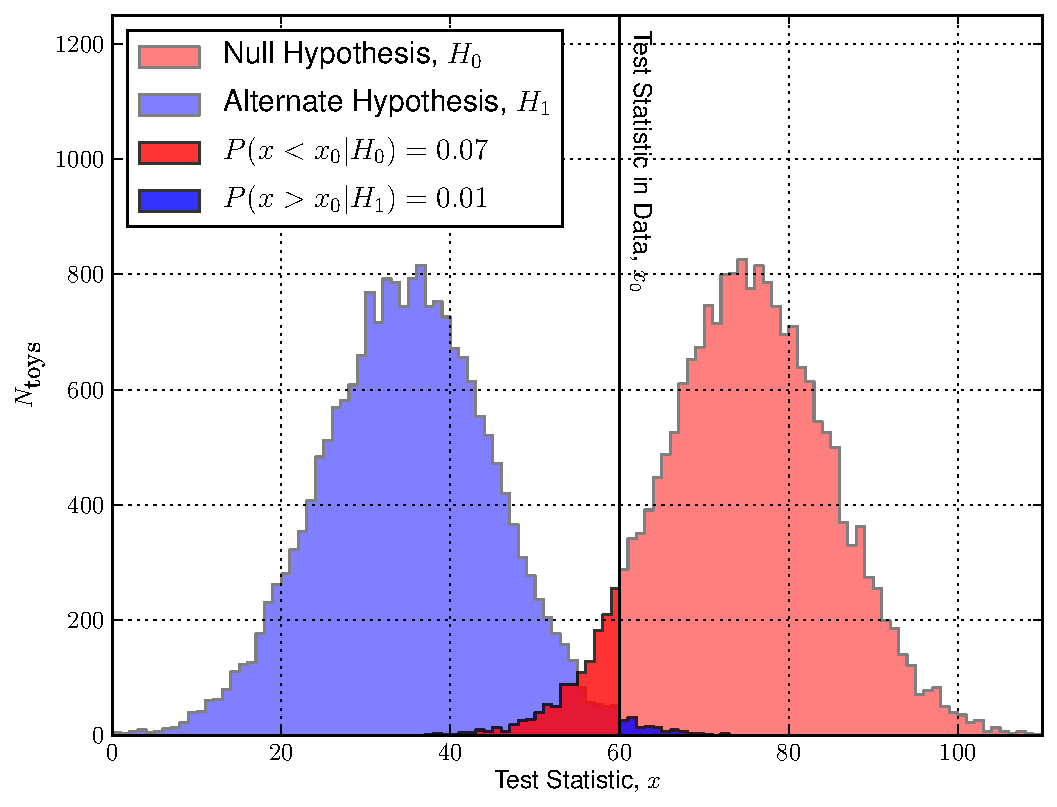
\includegraphics[width=0.49\textwidth]{fig/cls1}}
\subfloat[]{\label{fig:inter_cls_explain2}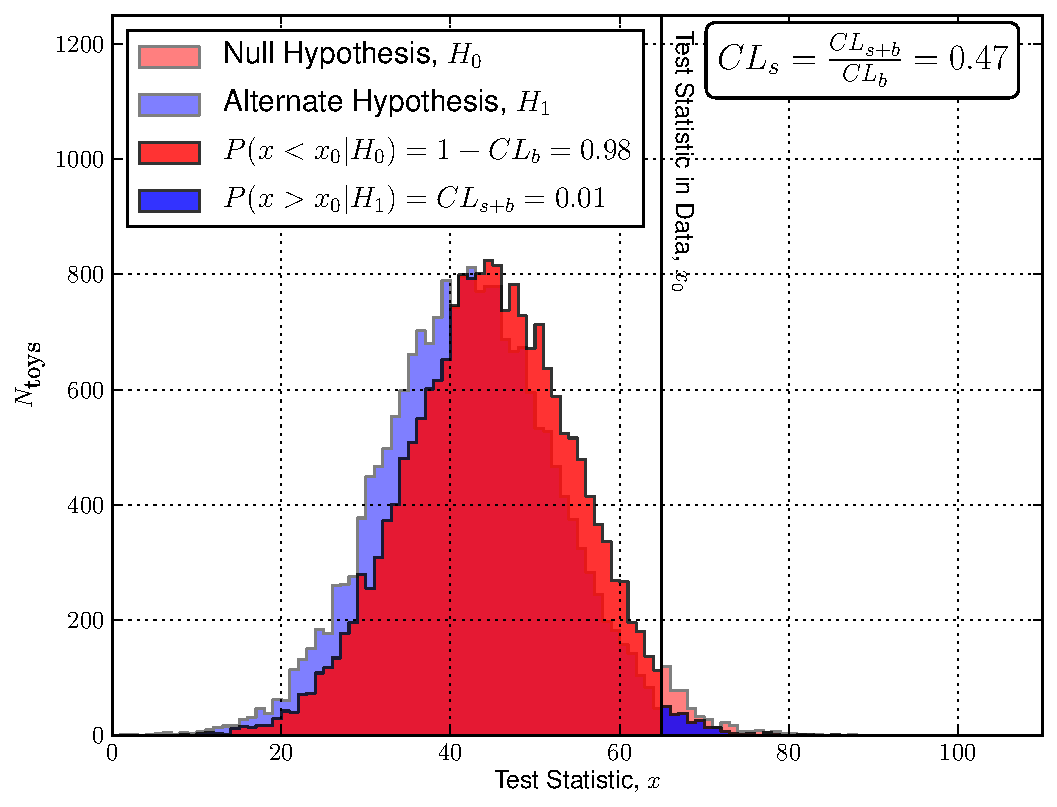
\includegraphics[width=0.49\textwidth]{fig/cls2}}
\caption[]{}
\label{fig:inter_cls_explain}
\end{figure}

\subsection{The \CLs Method}
One deficiency of the above method is that often the two hypotheses will not be
so well separated. This situation is shown in
Figure~\ref{fig:inter_cls_explain2}. In this case, the p-value for the alternate
hypothesis is small and so would result in an exclusion. This is undesirable
since the test statistic is clearly not sensitive enough to distinguish the two
hypotheses.

To address this problem, the \CLs hypothesis test may be used instead,
\begin{equation*}
\CLs = \frac{CL_{s+b}}{CL_{b}}
\end{equation*}
where, for the example shown in Figure~\ref{fig:inter_cls_explain2},
\begin{eqnarray*}
CL_{s+b} = P\left(x > x_0 | H_1\right)\\
CL_b = 1 - P\left(x < x_0 | H_0\right)
\end{eqnarray*}
where the null hypothesis now represents a background-only ($b$) scenario, and
the alternate, signal-plus-background ($s+b$). Using the \CLs to test the
alternate hypothesis, instead of a p-value, penalises cases where the test
statistic provides little sensitivity - since $CL_b$ will be large. For a 95\%
exclusion, $\CLs < 0.05$ is required, as before. \CLs may also be used to derive
an upper limit on some parameter by scanning through different values of the
parameter of interest in order to obtain a 95\% upper limit. This is known as
``hypothesis test inversion''.

Several additional details are relevant to the discussion here. Firstly, the toy
experiments used to generate distributions of the test statistic redice values
of the nuisance parameters around their expected values. The test statistic used
is the one-sided profile likelihood \cite{cl_computation, modified_frequentist, atlas_cms_higgs}.

\section{The Single Lepton Supersymmetry Search}
The full development of the likelihood function used to model the single lepton
supersymmetry search is covered in complete detail in
Appendix~\ref{sec:inter_1lepton}. In this section, only a few pertinent points
will be discussed. Firstly, the evaluation of model-dependent systematic effects
associated with the signal yield. Secondly, some discussion of validation work
performed to demonstrate that the statistical procedure and software
infrastructure are functioning as expected.

\subsection{Signal Systematics}
As can be seen in Table~\ref{tbl:inter_systematic_parameters}, a number of
nuisance parameters are assigned for systematic uncertainties affecting the
expected signal yield.

Both the luminosity estimate and the trigger efficiency are subject to
uncertainties which would effect the expected signal yield. Uncertainties of 4\%
and 1\% are assigned.

The signal efficiency will also be affected by the choice of \acp{PDF} in the
simulated samples and the calculation of the \ac{NLO} cross-sections. Whilst in
principal these would be expected to vary across the parameter space of a given
theoretical model, the complexity of the calculation involved in accurately
evaluating this systematic led us to assign a conservative 10\% systematic.

For the jet energy scale and \MET resolution uncertainty, these are calculated
as for the background case (see Sections~\ref{sec:susy_jes_uncertainty} and
\ref{sec:susy_metres_uncertainty}). These are calculated individually for
different signal hypotheses. As summary of all uncertainties assigned for the
signal efficiencies, along with their exact or approximate size, is shown in
Table~\ref{tbl:inter_signal_systematics}.

\ctable[
caption=Summary table of uncertainties related to the signal efficiency.,
mincapwidth=0.5\textwidth,
label=tbl:inter_signal_systematics,
pos=h
]{cc}{
}{\FL
Uncertainty & Value\ML
$\mathcal{L}$ & 4.5\%\NN
trigger efficiency & 1\%\NN
JES 5\% & Model dependent (10-15\% for \ac{CMSSM})\NN
PFMET resolution 10\%& Model dependent (0.5-15\% for \ac{CMSSM})\NN
PDF and NLO& 10\%\LL
}


\begin{figure}[h!]
\centering
\subfloat[]{\label{fig:inter_pl_80_400_syst}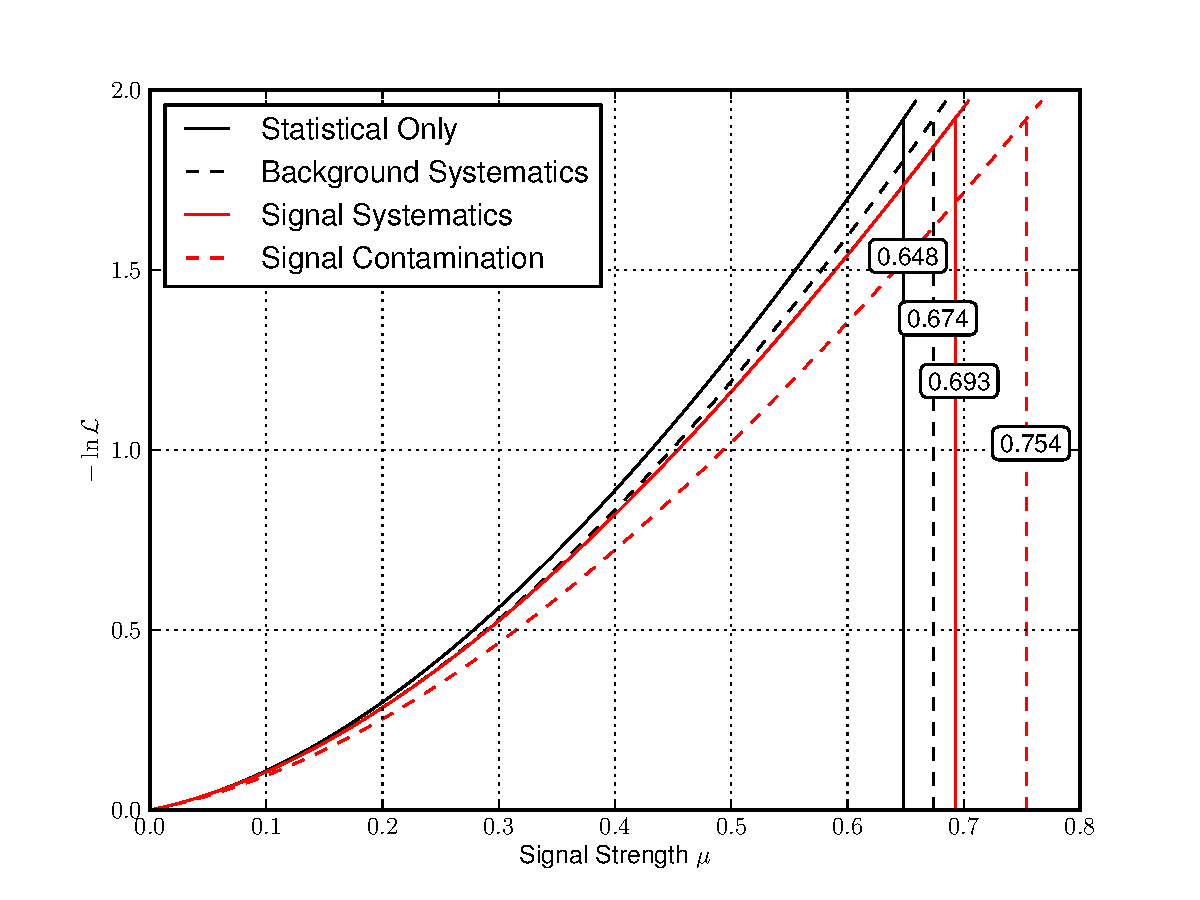
\includegraphics[width=0.47\textwidth]{fig/pl_systematics_80_400}}\quad
\subfloat[]{\label{fig:inter_pl_80_400_muon}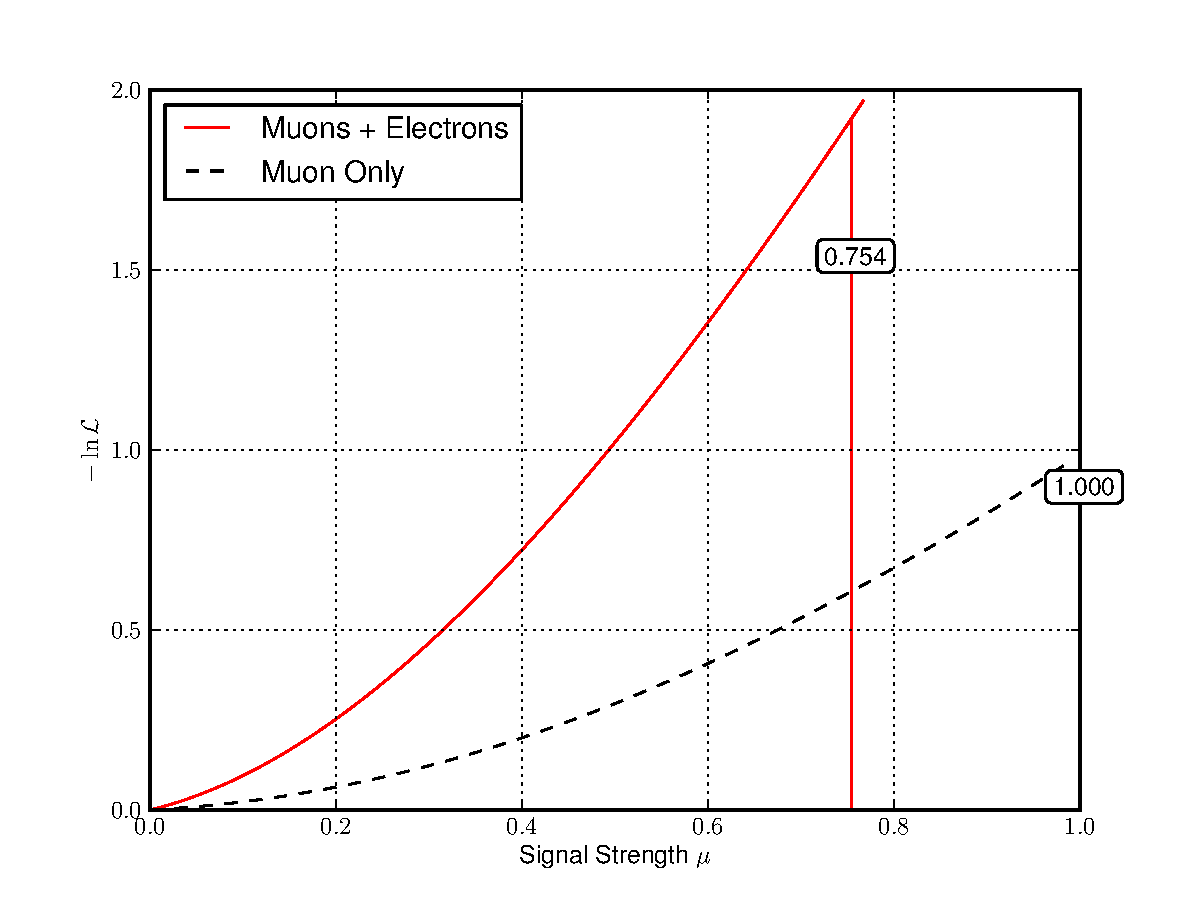
\includegraphics[width=0.47\textwidth]{fig/pl_muon_80_400}}
\caption[]{}
\label{fig:inter_pl}
\end{figure}

\begin{figure}[h!]
\centering
\subfloat[Statistical Uncertainties Only]{
  \label{fig:inter_cls_80_400_syst}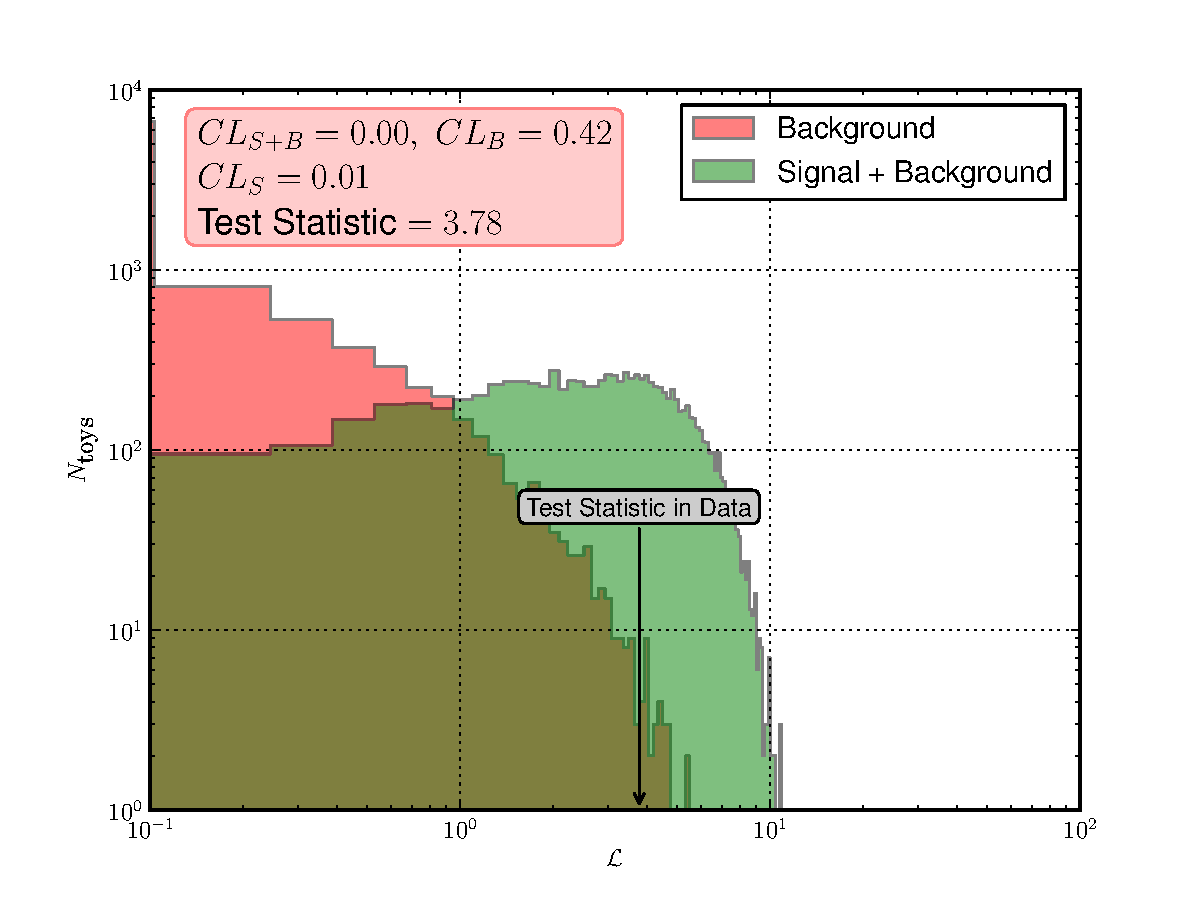
\includegraphics[width=0.47\textwidth]{fig/exp_muon_electron_80_400_bgsysts_no_sigsysts_no_sigcon_no}}\quad
\subfloat[Background Systematics]{
  \label{fig:inter_cls_80_400_muon}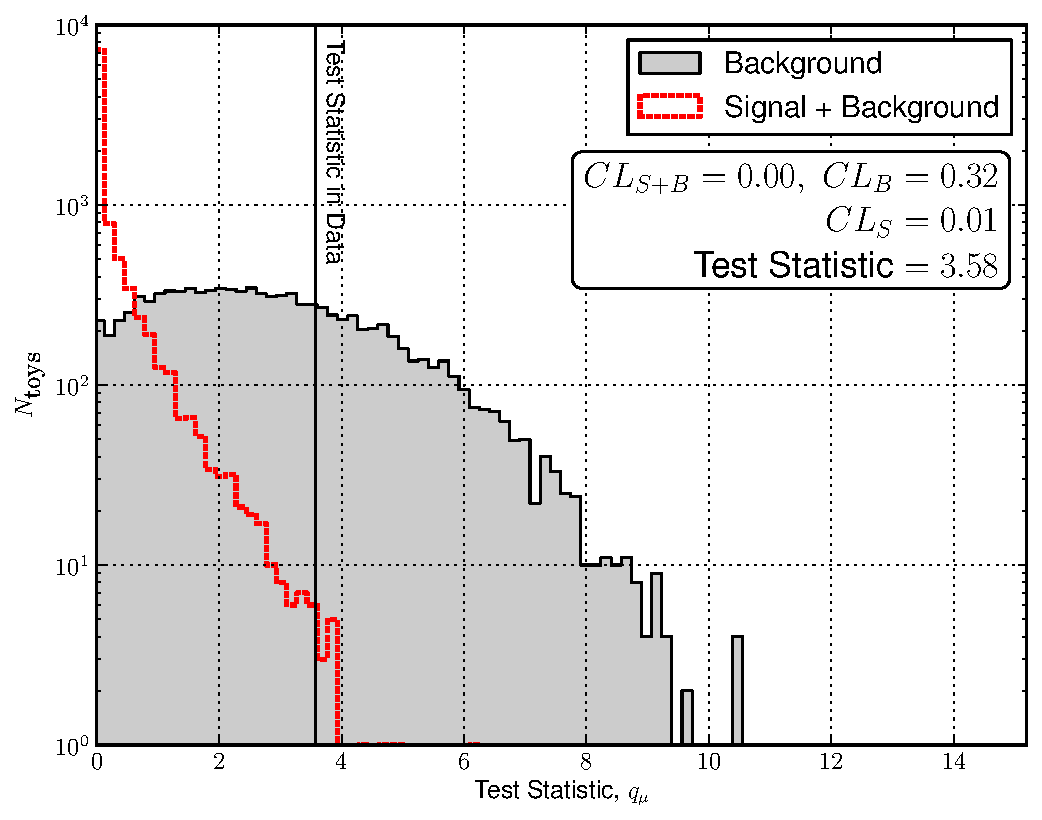
\includegraphics[width=0.47\textwidth]{fig/exp_muon_electron_80_400_bgsysts_yes_sigsysts_no_sigcon_no}}\\
\subfloat[Signal Systematics]{
  \label{fig:inter_cls_80_400_syst}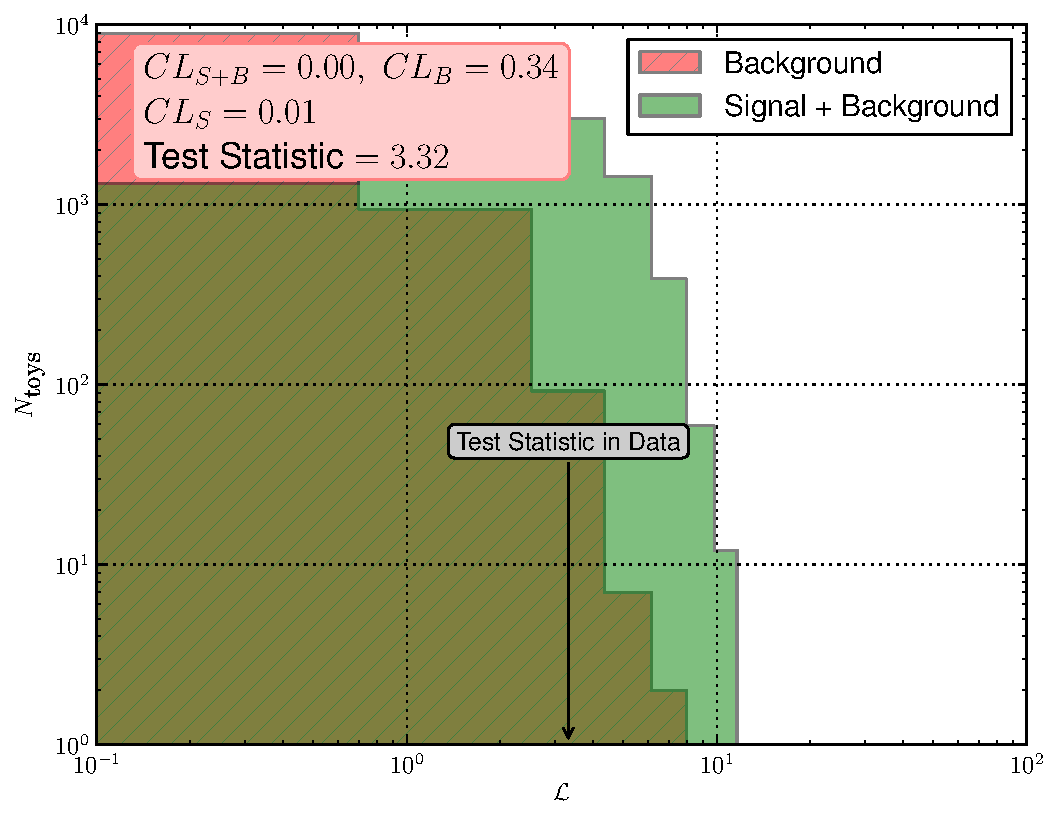
\includegraphics[width=0.47\textwidth]{fig/exp_muon_electron_80_400_bgsysts_yes_sigsysts_yes_sigcon_no}}\quad
\subfloat[Signal Contamination]{
  \label{fig:inter_cls_80_400_muon}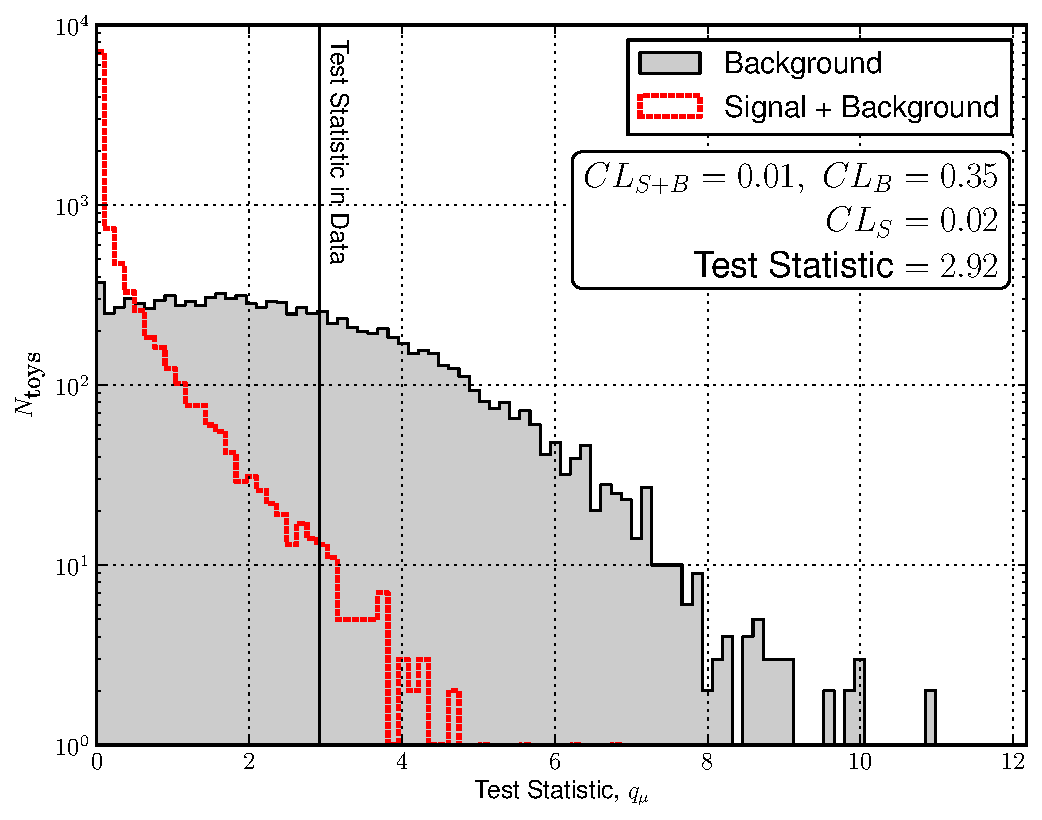
\includegraphics[width=0.47\textwidth]{fig/exp_muon_electron_80_400_bgsysts_yes_sigsysts_yes_sigcon_yes}}\\
\subfloat[Muon Channel Only]{
  \label{fig:inter_cls_80_400_muon}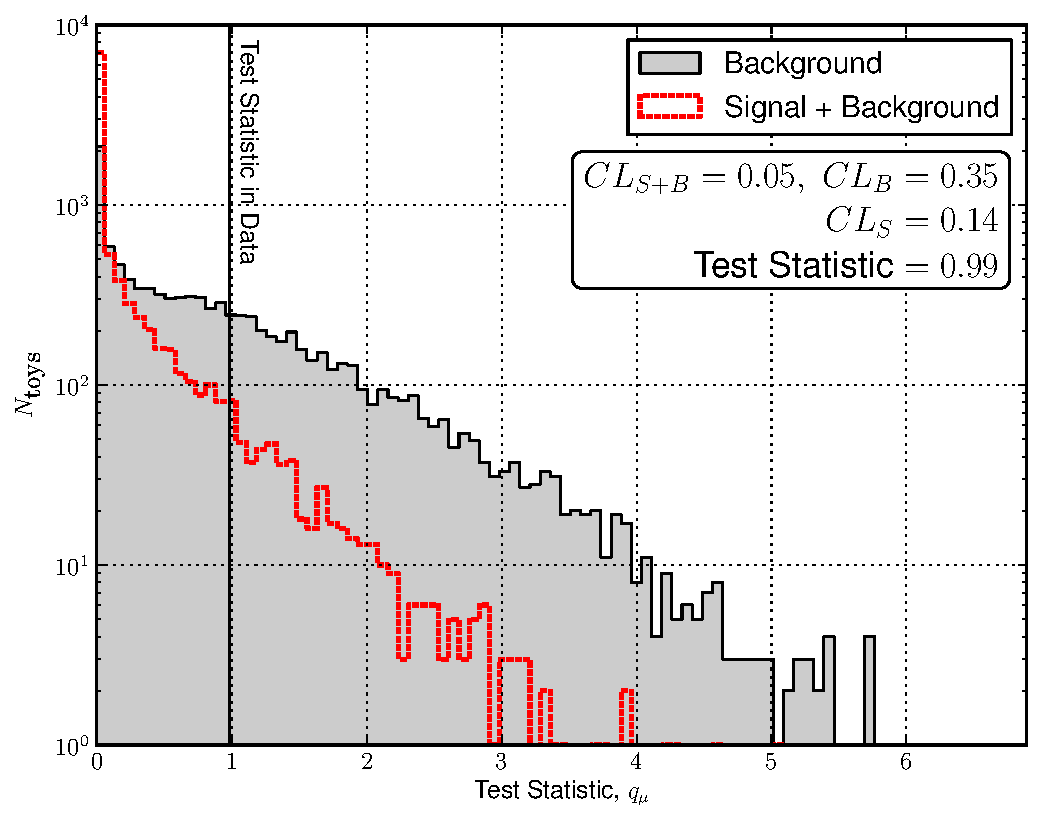
\includegraphics[width=0.47\textwidth]{fig/exp_muon_80_400_bgsysts_yes_sigsysts_yes_sigcon_yes}}
\caption[]{}
\label{fig:inter_cls}
\end{figure}

\subsection{Validation}
To validate the correct working of the model, a number of cross-checks were
performed. Firstly, the Profile Likelihood and \CLs methods were compared and
found to agree. In general, the \CLs method is expected to be more conservative
in convering the full range of the nuisance parameters in the model.

To see how the Profile Likelihood and \CLs results change with modifications to
the likelihood function, a representative point in the \ac{mSUGRA} plane
($\tan\beta=10$, $A_0=0$, $\mu>0$) are chosen. These are $(m_0, m_{\frac{1}{2}})
= (80, 400)$, close to the edge of the region excluded by data (the point $(m_0,
m_{\frac{1}{2}}) = (80, 240)$ can be seen in
Section~\ref{sec:app_inter_validation}).

The Profile Likelihood function for this point can be seen in
Figure~\ref{fig:inter_pl}. It can be seen that adding the various systematic
effects to the model, and also removing the electron channel appear to have the
expected effect on the resulting upper limit.

The distributions of the test statistic used to calculate \CLs are shown in
Figure~\ref{fig:inter_cls}. Again the effects of adding systematic parameters
and removing the electron channel appears to have the expected effect on
\CLs.


\section{Results}
The likelihood model is used to provide interpretation within the context of two
\ac{NP} models: \ac{mSUGRA} and the \Ttwott simplified model described in
Section~TODO.

\begin{figure}[h!]
\centering
\subfloat[]{\label{fig:inter_msugra_mu_eff250}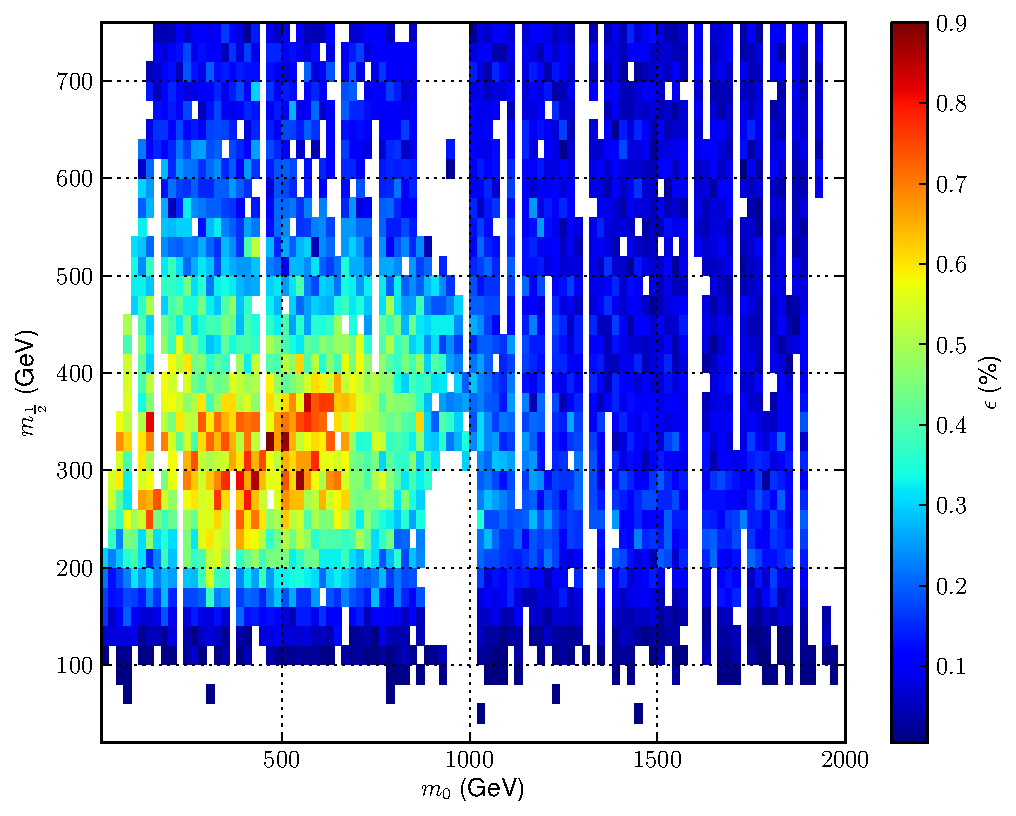
\includegraphics[width=0.49\textwidth]{fig/msugra_muons_eff_250}}
\subfloat[]{\label{fig:inter_msugra_mu_eff350}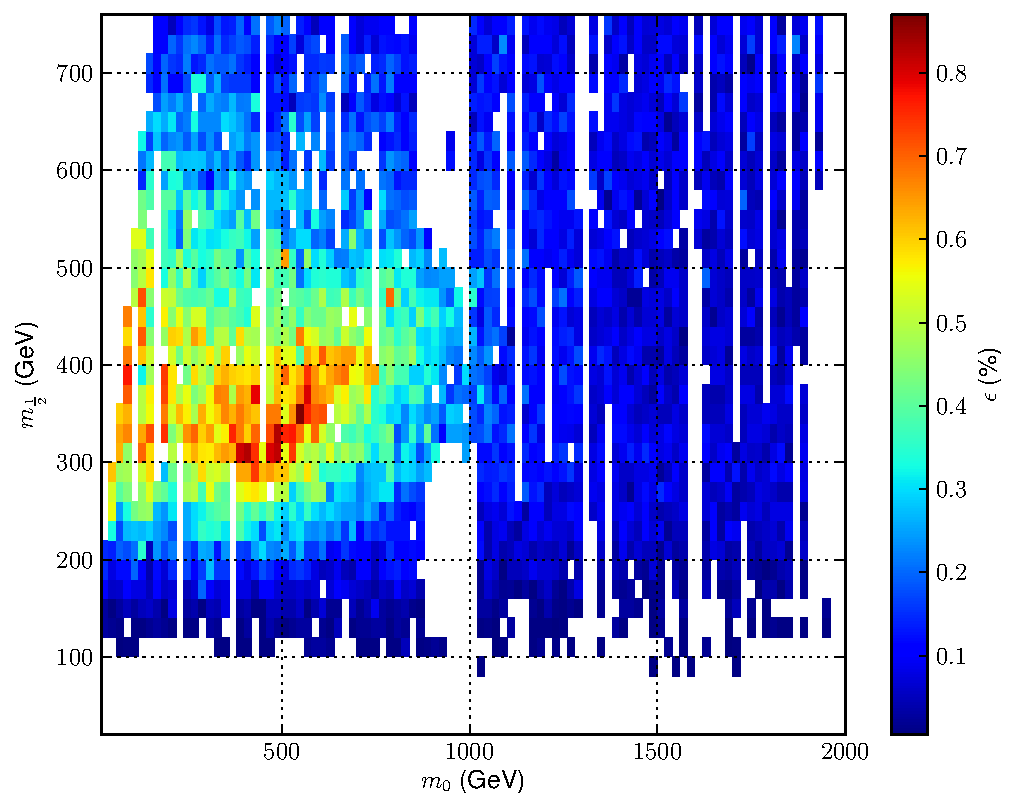
\includegraphics[width=0.49\textwidth]{fig/msugra_muons_eff_350}}\\
\subfloat[]{\label{fig:inter_msugra_mu_eff450}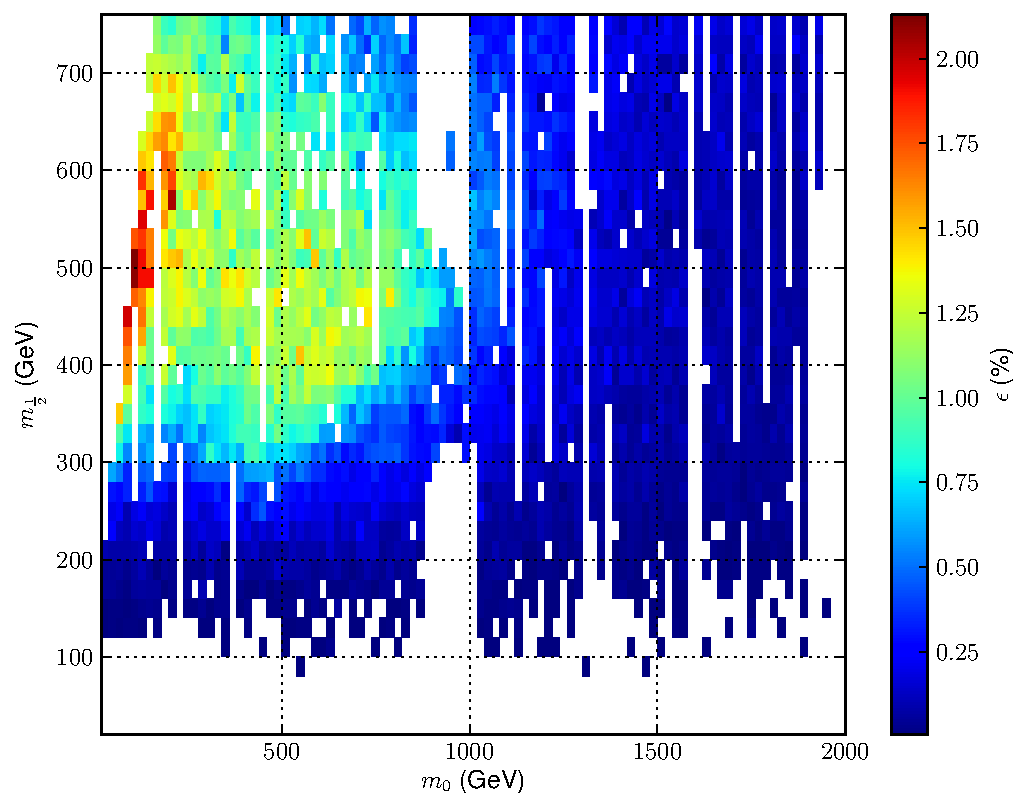
\includegraphics[width=0.49\textwidth]{fig/msugra_muons_eff_450}}
\subfloat[]{\label{fig:inter_msugra_mu_efftot}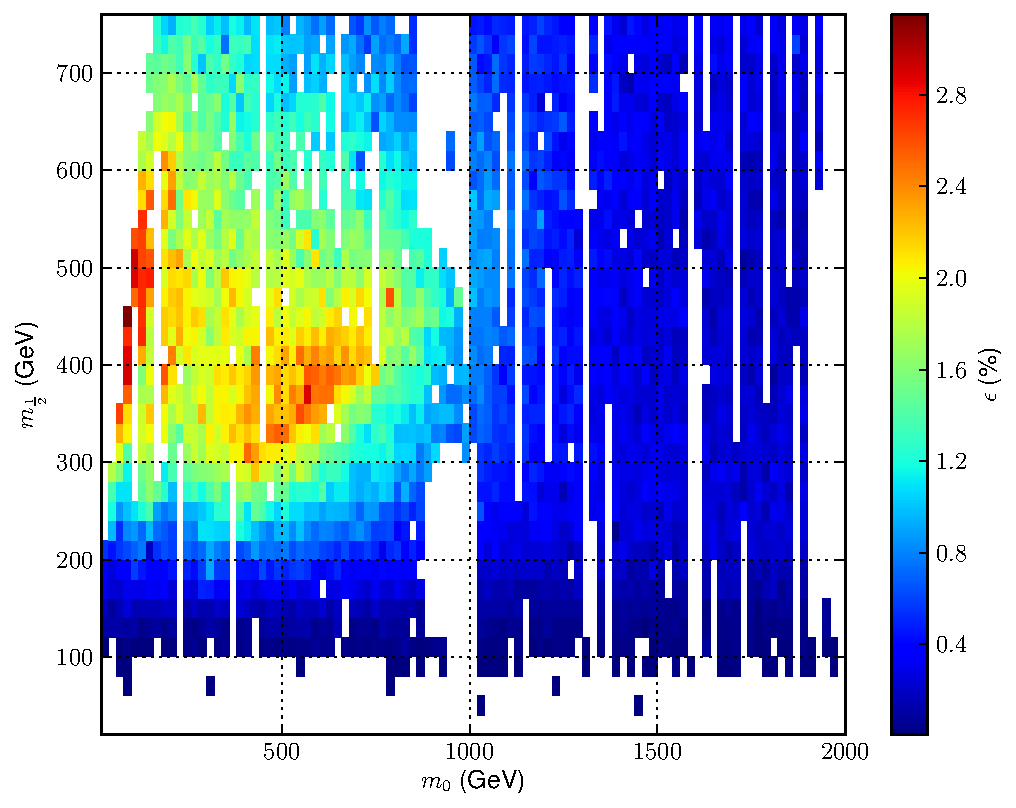
\includegraphics[width=0.49\textwidth]{fig/msugra_muons_eff_total}}
\caption[]{}
\label{fig:inter_msugra_mu}
\end{figure}

\begin{figure}[h!]
\centering
\subfloat[]{\label{fig:inter_msugra_el_eff250}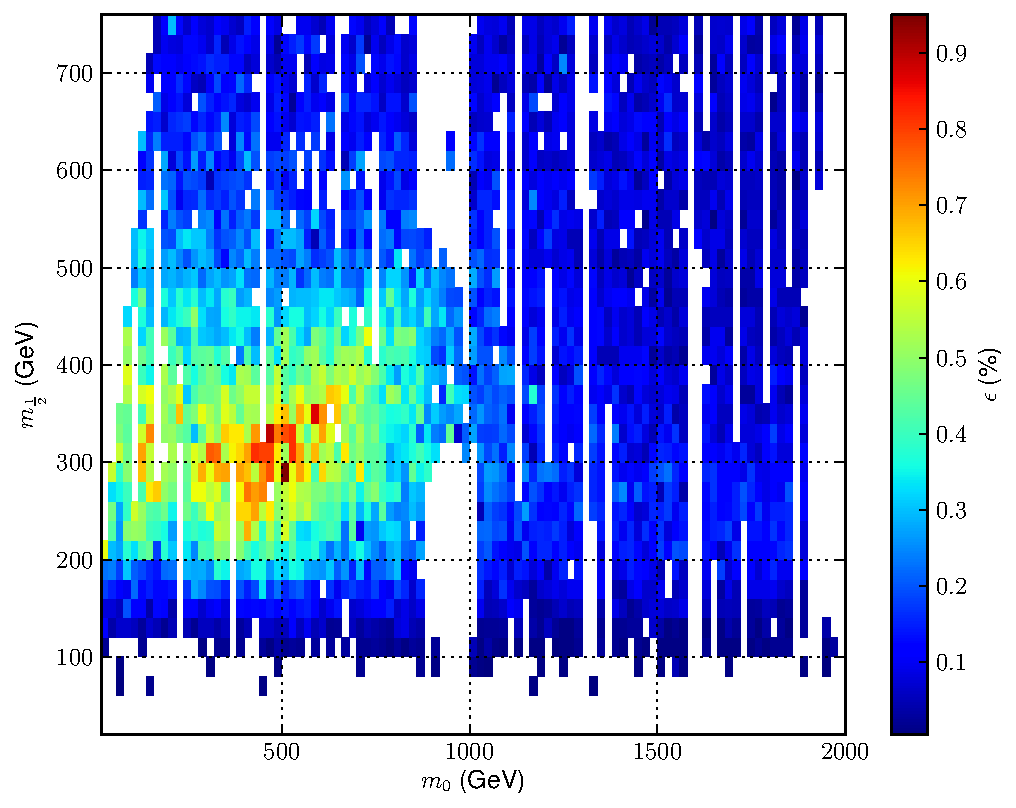
\includegraphics[width=0.49\textwidth]{fig/msugra_electrons_eff_250}}
\subfloat[]{\label{fig:inter_msugra_el_eff350}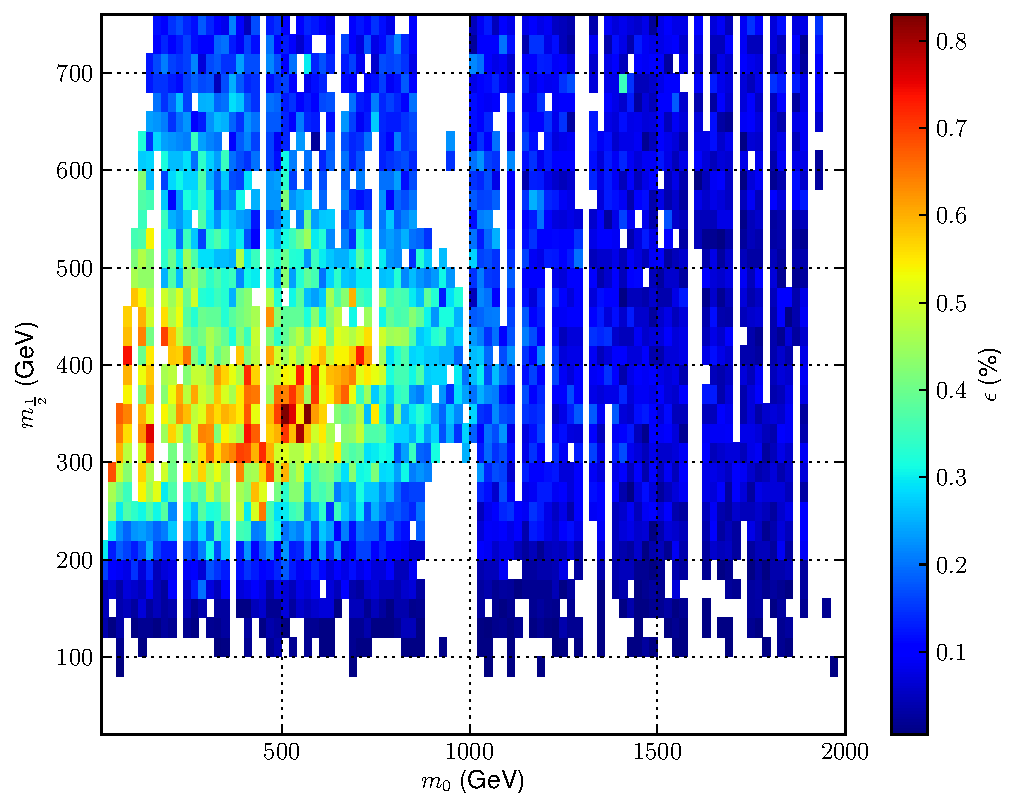
\includegraphics[width=0.49\textwidth]{fig/msugra_electrons_eff_350}}\\
\subfloat[]{\label{fig:inter_msugra_el_eff450}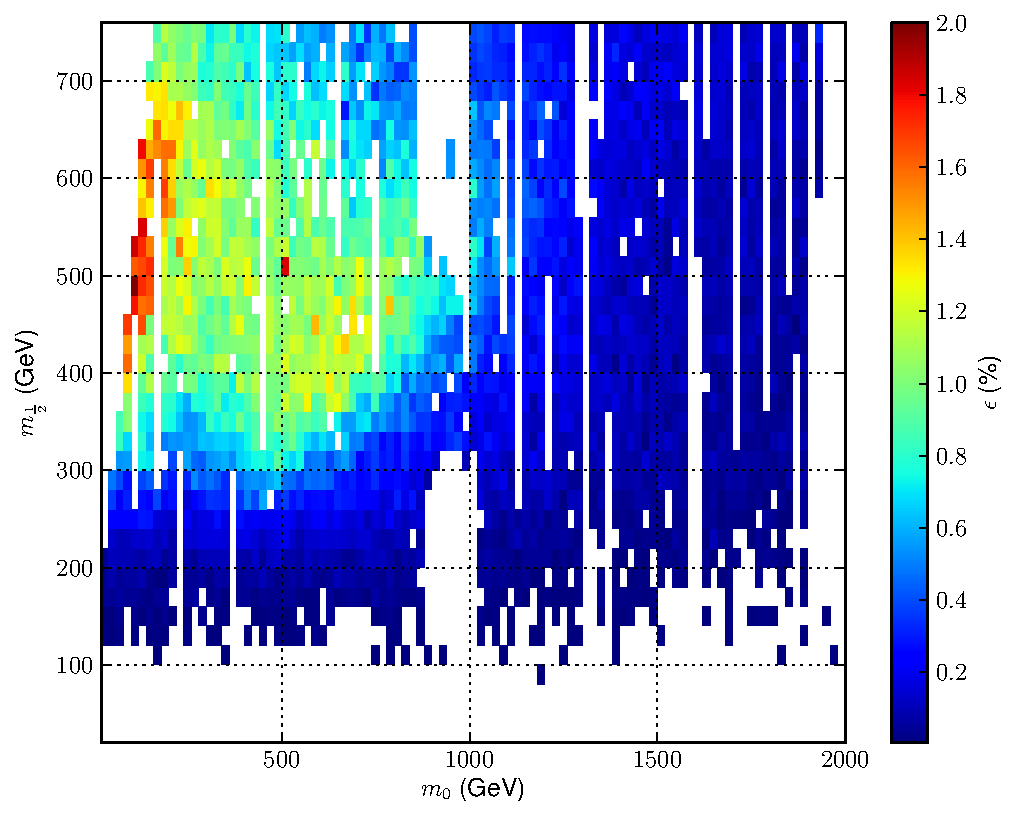
\includegraphics[width=0.49\textwidth]{fig/msugra_electrons_eff_450}}
\subfloat[]{\label{fig:inter_msugra_el_efftot}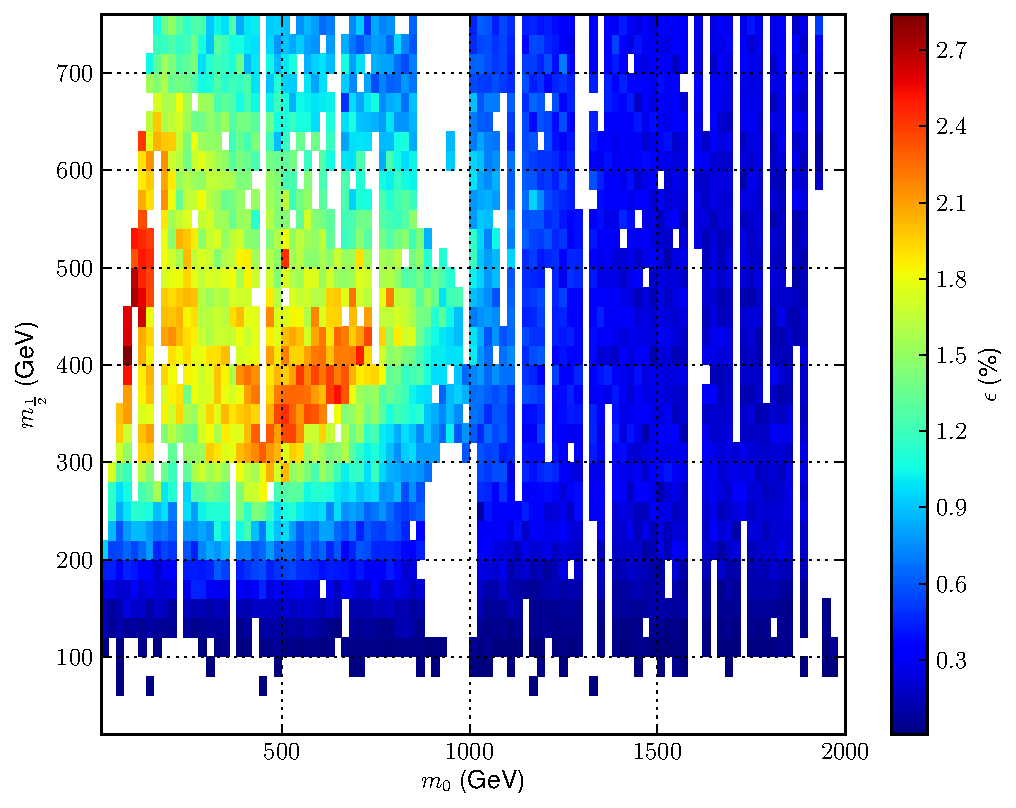
\includegraphics[width=0.49\textwidth]{fig/msugra_electrons_eff_total}}
\caption[]{}
\label{fig:inter_msugra_el}
\end{figure}

\begin{figure}[h!]
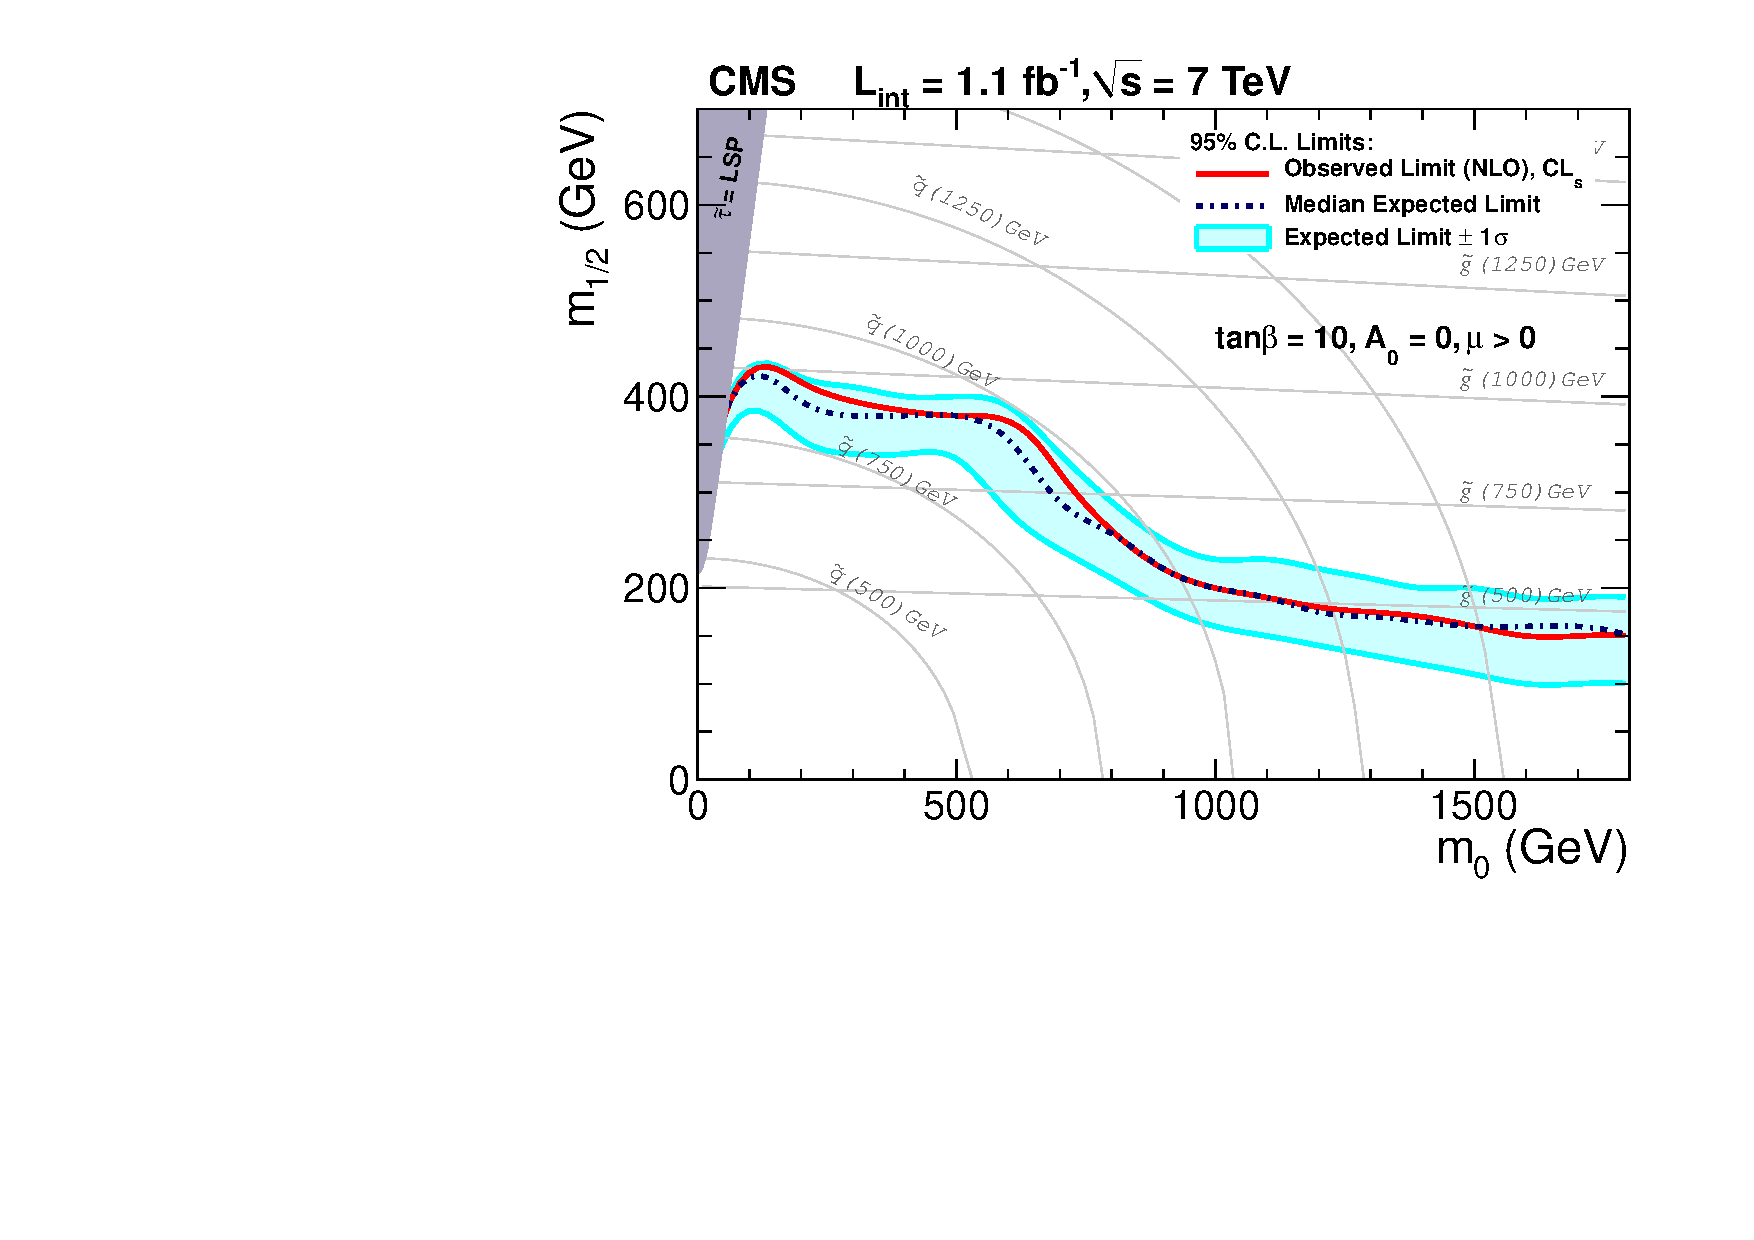
\includegraphics[width=\textwidth]{fig/RA4_ExclusionLimit_tanb10}
\caption[]{}
\label{fig:inter_msugra_exclusion}
\end{figure}

\subsection{\ac{CMSSM}}
The \ac{CMSSM} was previously described in Section~\ref{sec:cmssm}. As explained
previously, the \ac{CMSSM} makes a number of somewhat arbitrary choices which
restrict the \ac{SUSY} toplogies signatures it is able to encompass. Whilst
these make it relatively undesirable as a framework for theoretical
interpretation, it is nonetheless useful as a common yardstick by which to
compare experiments and searches.

The \ac{CMSSM} results are presented as a 95\% exclusion in a two-dimensional
plane of the parameter space where the two mass parameters, \Mzero and \Mhalf,
are allowed to vary. Other parameters are fixed as follows: $\Azero = 0$,
$\tanbeta = 10$ and $\mu > 0$.

\subsubsection{Technical Details}
The likelihood function detailed in Section~\ref{sec:inter_1lepton} takes as
input the signal efficiencies for each bin of \STlep. In the case of the
\ac{CMSSM}, these must be evaluated for each point $(\Mzero, \Mhalf)$. These are
evaluated using the same analysis procedure as used for the data and \ac{SM}
monte carlo samples. The \ac{CMSSM} sample is produced using the Pythia event
generator, with the two mass parameters varied independently in steps of
\unit{20}{\GeV} to produce a grid. For each grid point, 10000 events were
generated. Due to the large number of events, the detector response was not
processed with the full \ac{GEANT} reconstruction software but instead with a
faster, parameterised simulation tool. This has been extensively validated and
tuned against the full detector simulation and shown to give adequate results
for many analyses.

Having evaluated the efficiencies per \STlep bin for each \ac{CMSSM} grid point,
the \ac{NLO} cross-sections were calculated using the PROSPINO package
\cite{prospino}. These were then input to the limit code, along with the
required uncertainties and model-independent parameters.

\subsubsection{Efficiencies}
The efficiency per \STlep bin of the analysis selection as a function of the
\ac{CMSSM} parameter space is shown in Figures~\ref{fig:inter_msugra_mu} and
\ref{fig:inter_msugra_el} for muons and electrons respectively. The ``holes'' in
the \ac{mSUGRA} sample are due to incomplete data samples at the time of
publication.

The efficiencies give a good indication of the efficiency of the analysis in
different regions of the parameter space. Firstly, it can be seen that
regardless of the \STlep bin, significant efficiency is achieved only for values
of $\Mzero < \unit{1000}{\GeV}$. The correlation of \STlep and \Mhalf should
also be noted, with the higher bins generally sensitive to larger values of
\Mhalf.

\subsubsection{Exclusion}
For consistency with other \ac{SUSY} searches at the \ac{LHC}, a limit has been
set using the \CLs method described in Section~\ref{sec:inter_cls}. Whilst it is
possible, to set an upper limit on the signal strength parameter, $\mu$, this
becomes highly computationally intensive. Instead, a simple exclusion was
produced assuming \ac{NLO} cross-sections. This is shown in
Figure~\ref{fig:inter_msugra_exclusion}. All terms discussed in
Section~\ref{sec:inter_1lepton} have been included. The expected limit and $\pm
1\sigma$ bands were evaluated by setting the observations for each bin to be
exactly that predicted from data.


\subsection{Simplified Models}
\subsubsection{Technical Details}
The simplified models described in Section~\ref{sec:sms} were simulated using
the Pythia generator by reusing supersymmetry subprocesses. The mass parameters
in each model were varied in steps. By varying the masses of the squark or
gluino, \ac{LSP} and other intermediate particles, a grid of simplified model
points is created. These are then processed further as for the \ac{CMSSM}.

\subsection{\TthreeW}
\begin{figure}[h!]
\centering
\subfloat[]{\label{fig:inter_t3w_mu_efftot}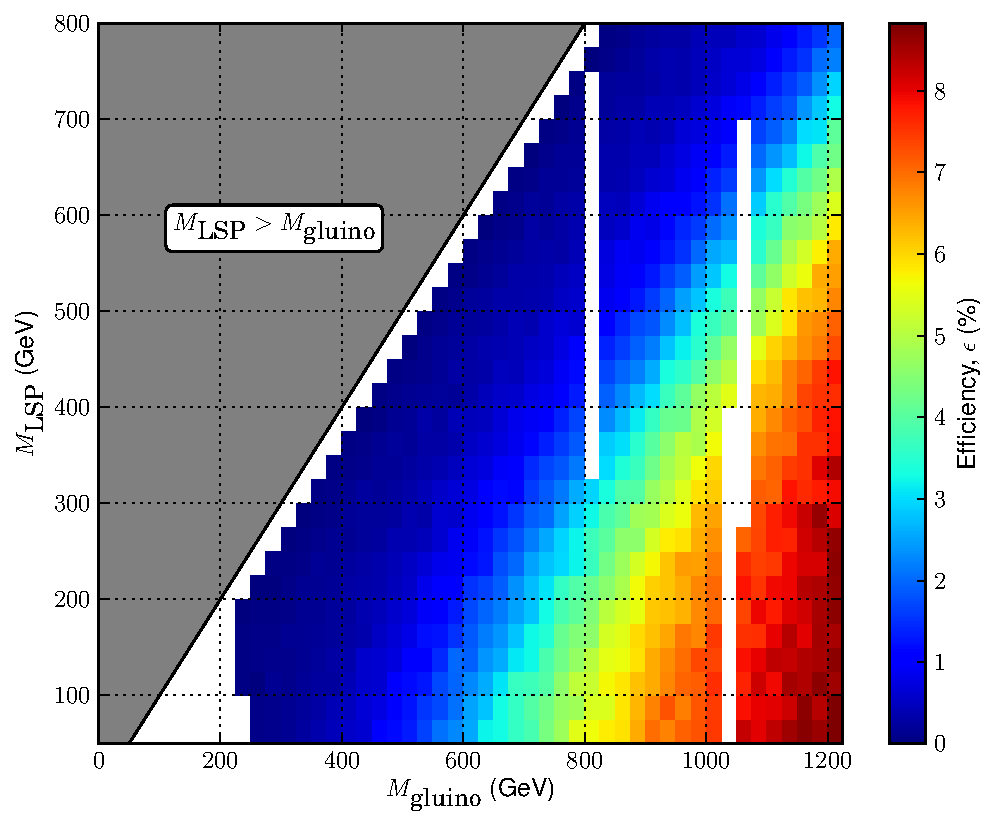
\includegraphics[width=0.49\textwidth]{fig/t3w_0p25_muons_eff_total}}
\subfloat[]{\label{fig:inter_t3w_mu_efftot}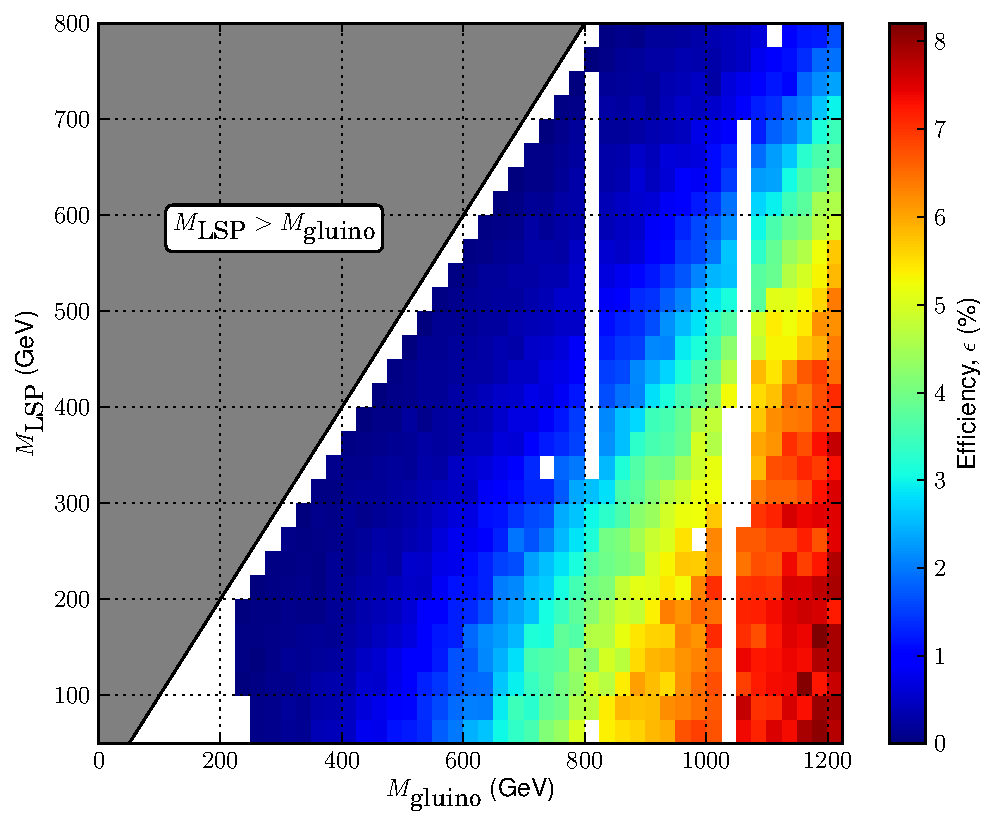
\includegraphics[width=0.49\textwidth]{fig/t3w_0p25_electrons_eff_total}}\\
\subfloat[]{\label{fig:inter_t3w_mu_efftot}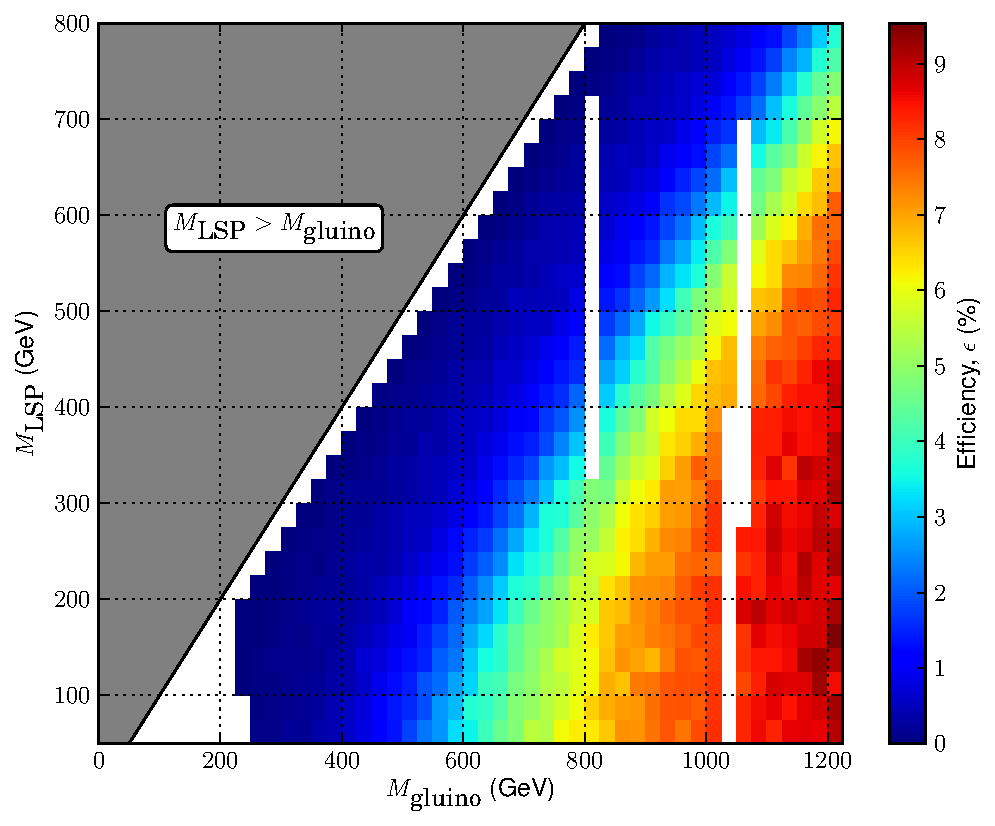
\includegraphics[width=0.49\textwidth]{fig/t3w_0p50_muons_eff_total}}
\subfloat[]{\label{fig:inter_t3w_mu_efftot}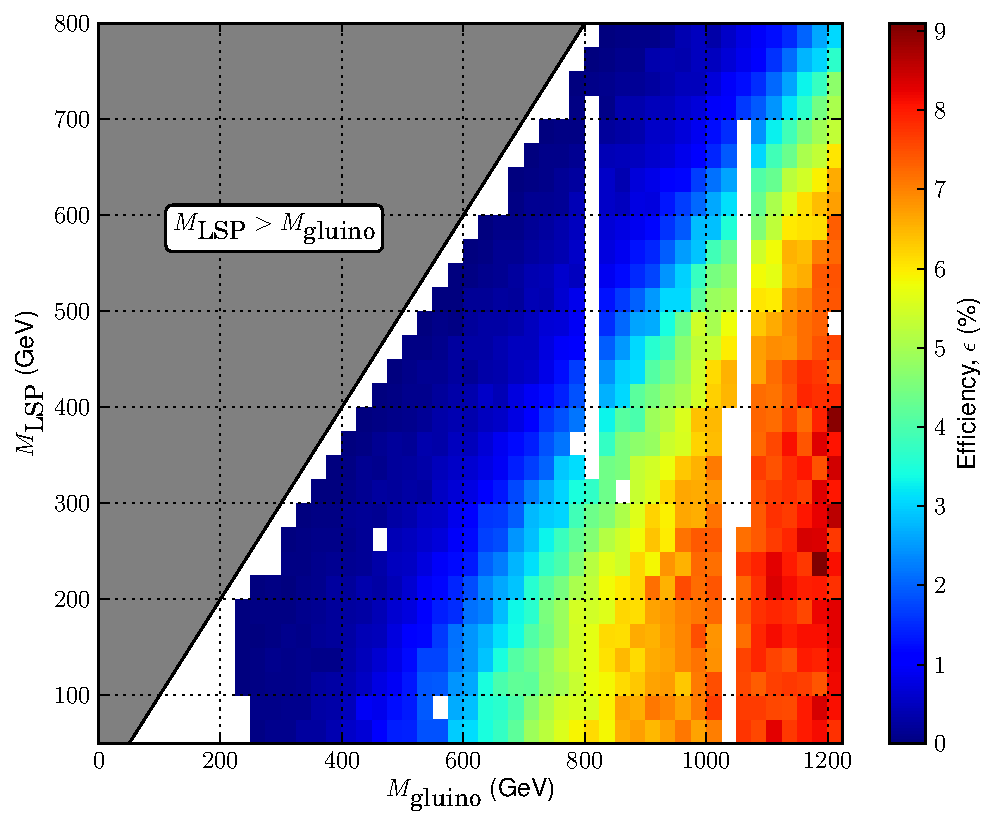
\includegraphics[width=0.49\textwidth]{fig/t3w_0p50_electrons_eff_total}}\\
\subfloat[]{\label{fig:inter_t3w_mu_efftot}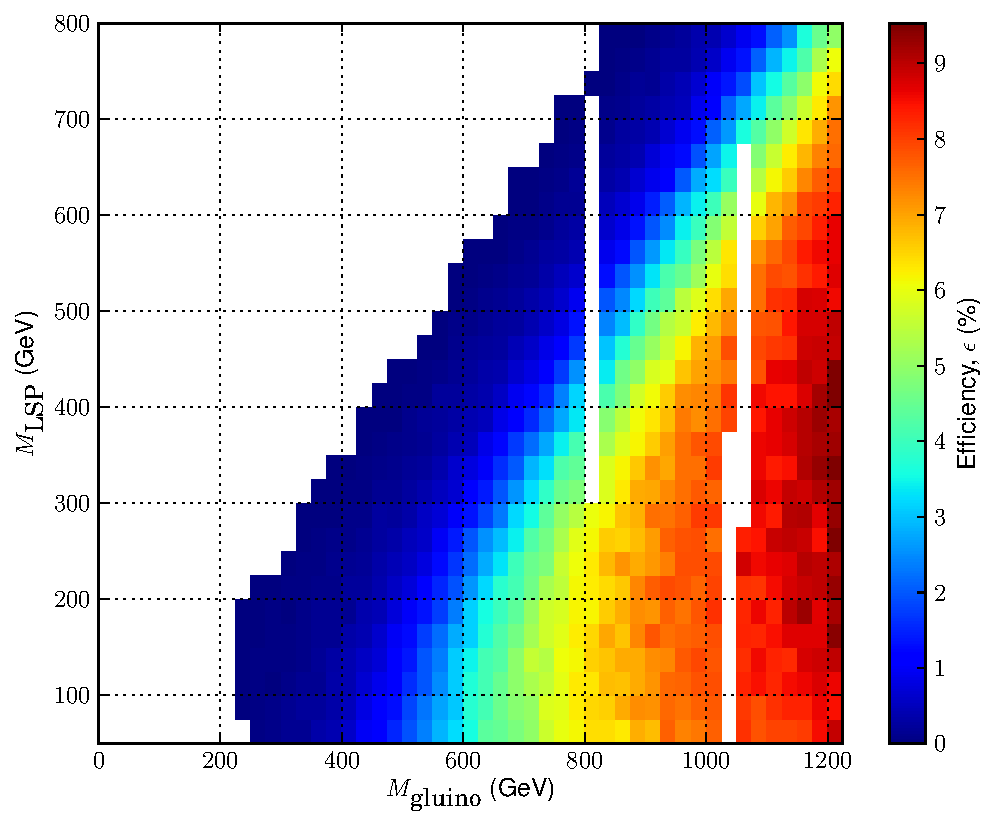
\includegraphics[width=0.49\textwidth]{fig/t3w_0p75_muons_eff_total}}
\subfloat[]{\label{fig:inter_t3w_mu_efftot}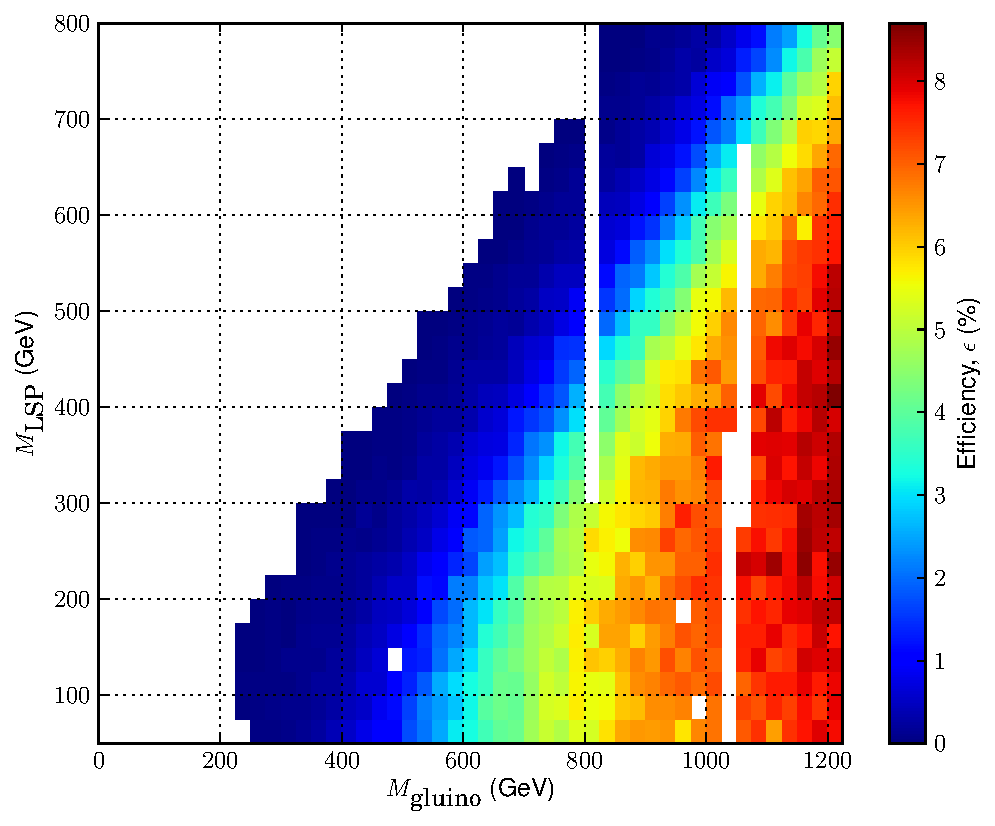
\includegraphics[width=0.49\textwidth]{fig/t3w_0p75_electrons_eff_total}}
\caption[]{}
\label{fig:inter_t3w_eff}
\end{figure}

\begin{figure}[h!]
\centering
\subfloat[]{\label{fig:inter_t3w_0p25_limit}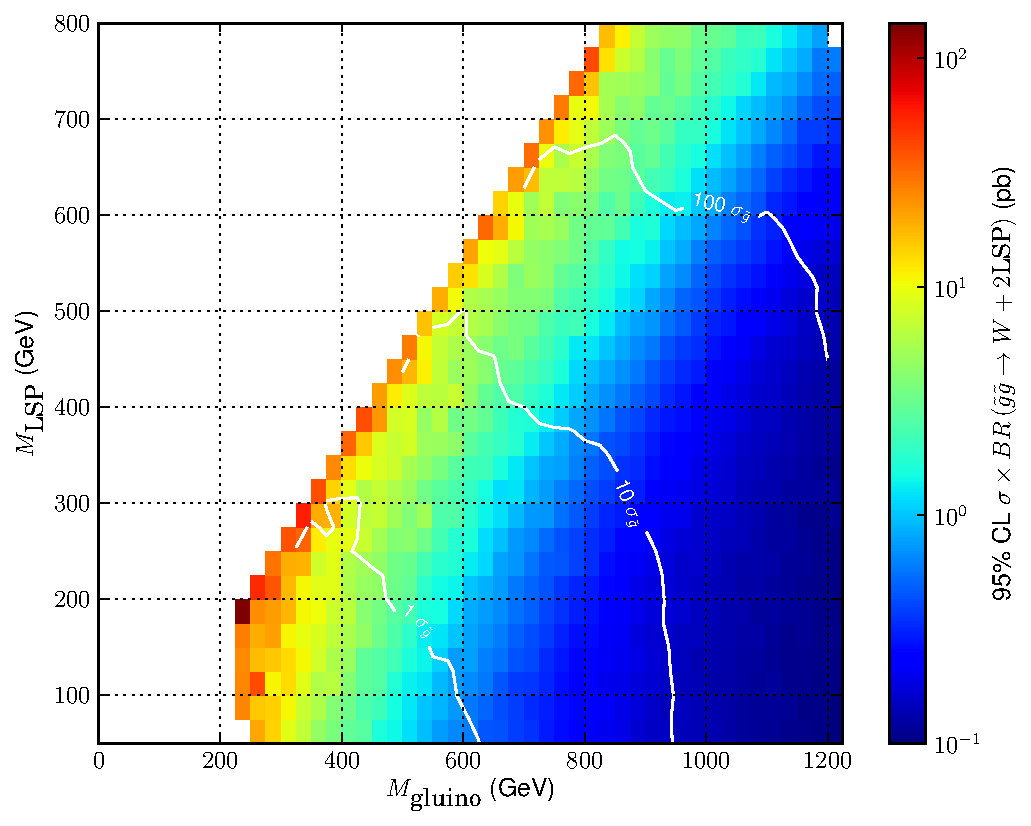
\includegraphics[width=0.49\textwidth]{fig/t3w_0p25_limit}}
\subfloat[]{\label{fig:inter_t3w_0p25_limit_1d}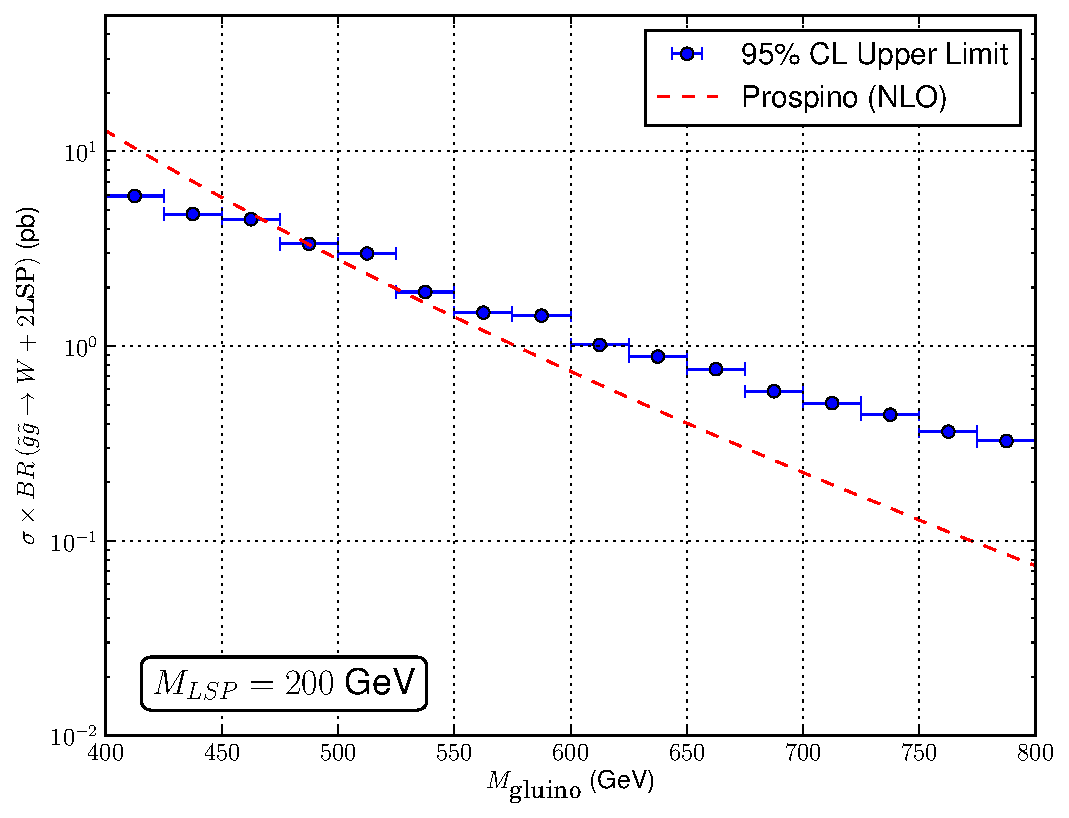
\includegraphics[width=0.49\textwidth]{fig/t3w_0p25_limit_1d}}
\caption[]{}
\label{fig:inter_t3w_0p25}
\end{figure}

\begin{figure}
\centering
\subfloat[]{\label{fig:inter_t3w_0p50_limit}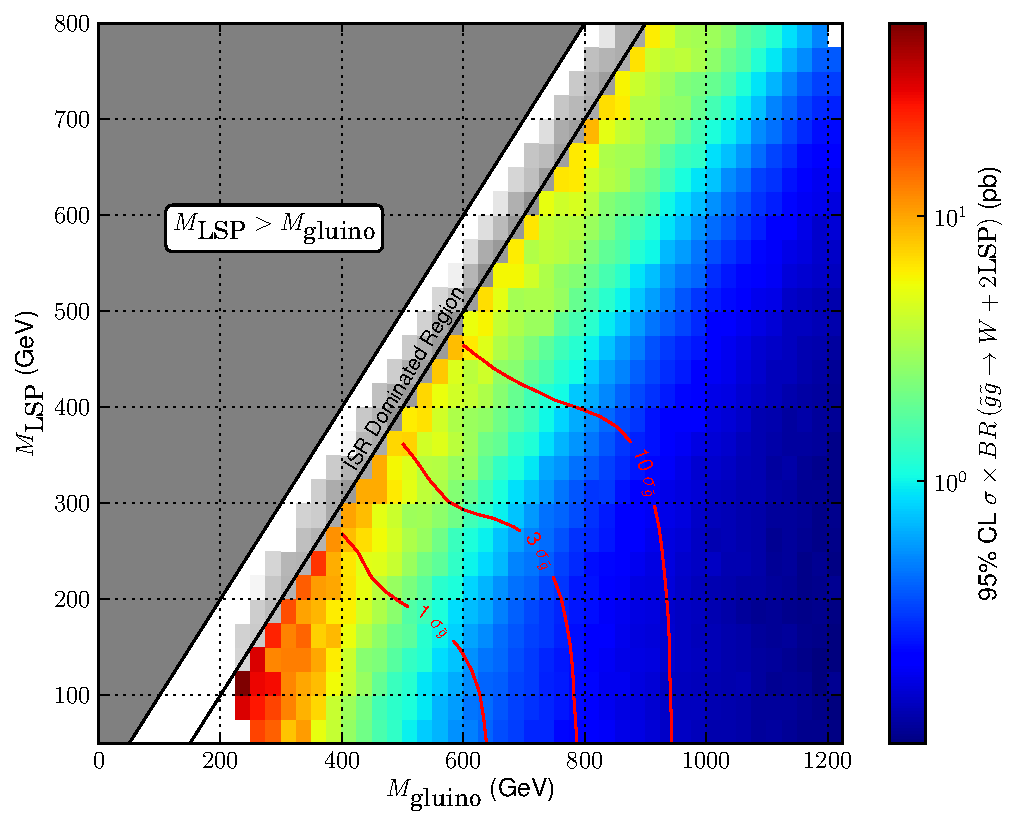
\includegraphics[width=0.49\textwidth]{fig/t3w_0p50_limit}}
\subfloat[]{\label{fig:inter_t3w_0p50_limit_1d}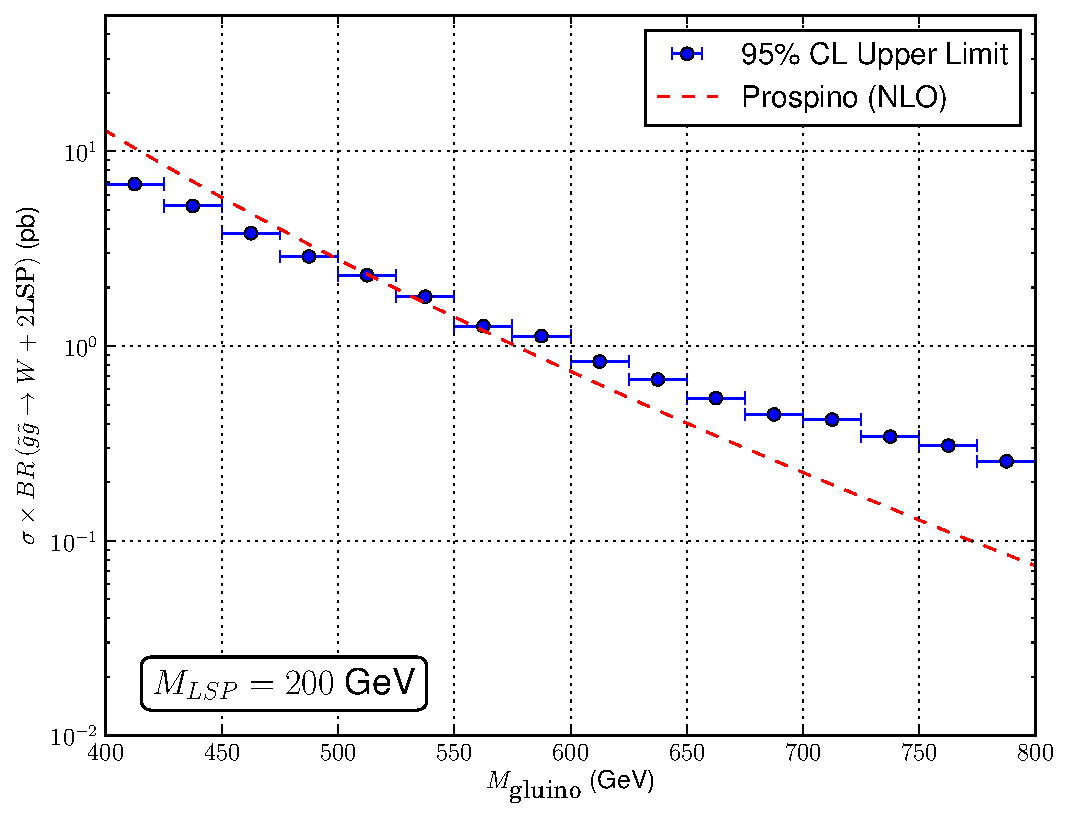
\includegraphics[width=0.49\textwidth]{fig/t3w_0p50_limit_1d}}
\caption[]{}
\label{fig:inter_t3w_0p50}
\end{figure}

\begin{figure}
\centering
\subfloat[]{\label{fig:inter_t3w_0p75_limit}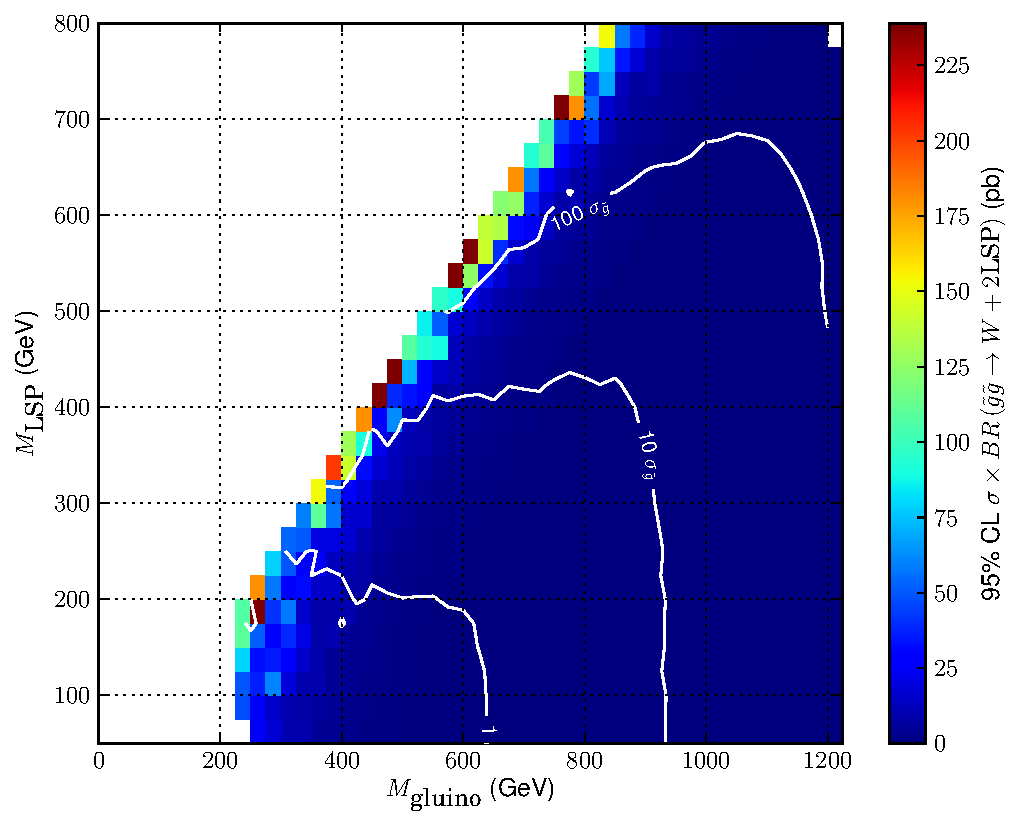
\includegraphics[width=0.49\textwidth]{fig/t3w_0p75_limit}}
\subfloat[]{\label{fig:inter_t3w_0p75_limit_1d}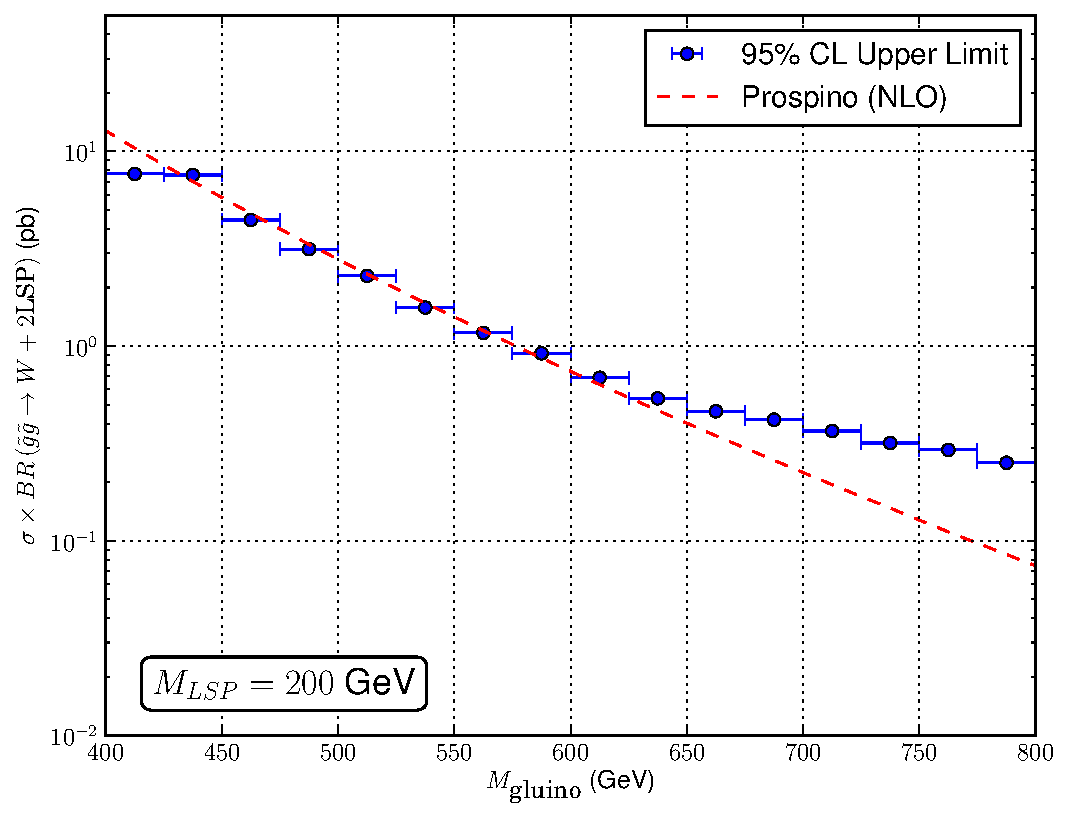
\includegraphics[width=0.49\textwidth]{fig/t3w_0p75_limit_1d}}
\caption[]{}
\label{fig:inter_t3w_0p75}
\end{figure}

\subsubsection{\Ttwott}
The efficiency per \STlep bin with respect to the \Ttwott parameter
space is shown in Figures~\ref{fig:inter_t2tt_mu} and \ref{fig:inter_t2tt_el}
respectively.

For the \Ttwott result it is desirable to have not only an exclusion plot, but
an upper limit on the cross-section. To reduce computation time, the limit was
set using a Profile Likelihood method (see
Section~\ref{sec:inter_profile_likelihood}). In addition, the uncertainties on
the signal efficiency and the signal contamination were not included. The upper
limit on the \Ttwott cross-section is shown in
Figure~\ref{fig:inter_t2tt_limit}. The contours show this limit as a function of
the expected stop production cross-section calculated using Prospino (TODO check
and cite). Figure~\ref{fig:inter_t2tt_limit_1d} shows the upper limit in
one-dimension for $M_{LSP} = \unit{50}{\GeV}$.

\begin{figure}[h!]
\centering
\subfloat[]{\label{fig:inter_t2tt_mu_eff250}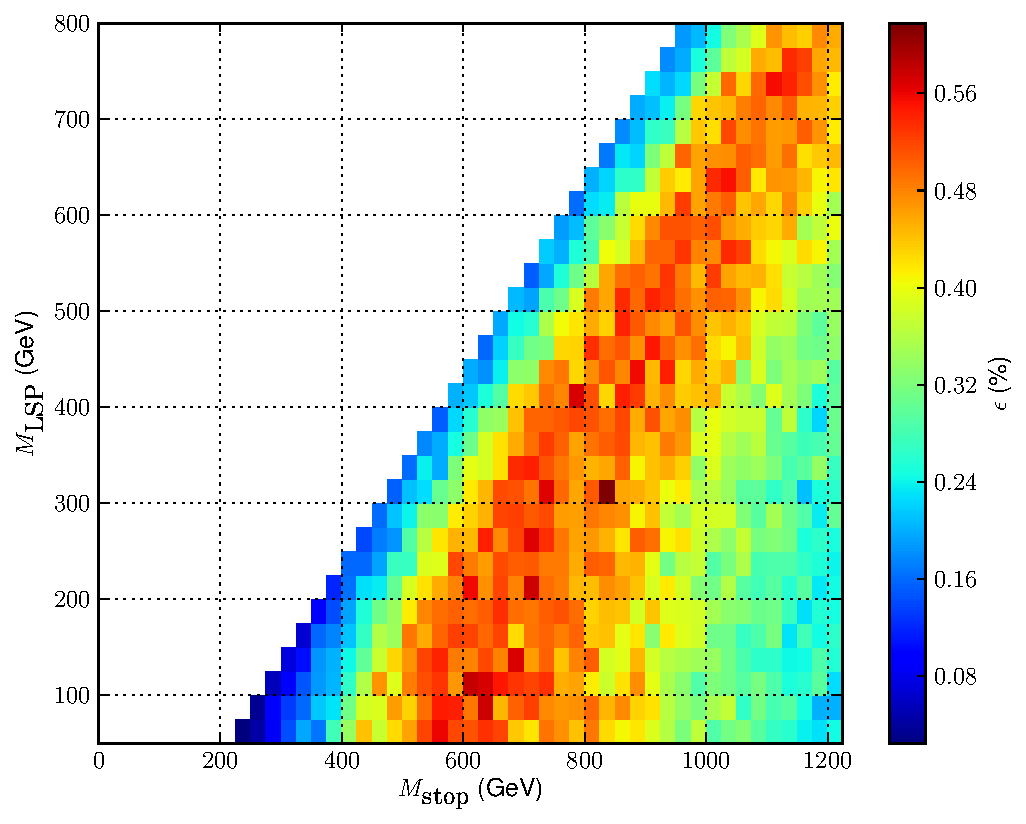
\includegraphics[width=0.49\textwidth]{fig/t2tt_muons_eff_250}}
\subfloat[]{\label{fig:inter_t2tt_mu_eff350}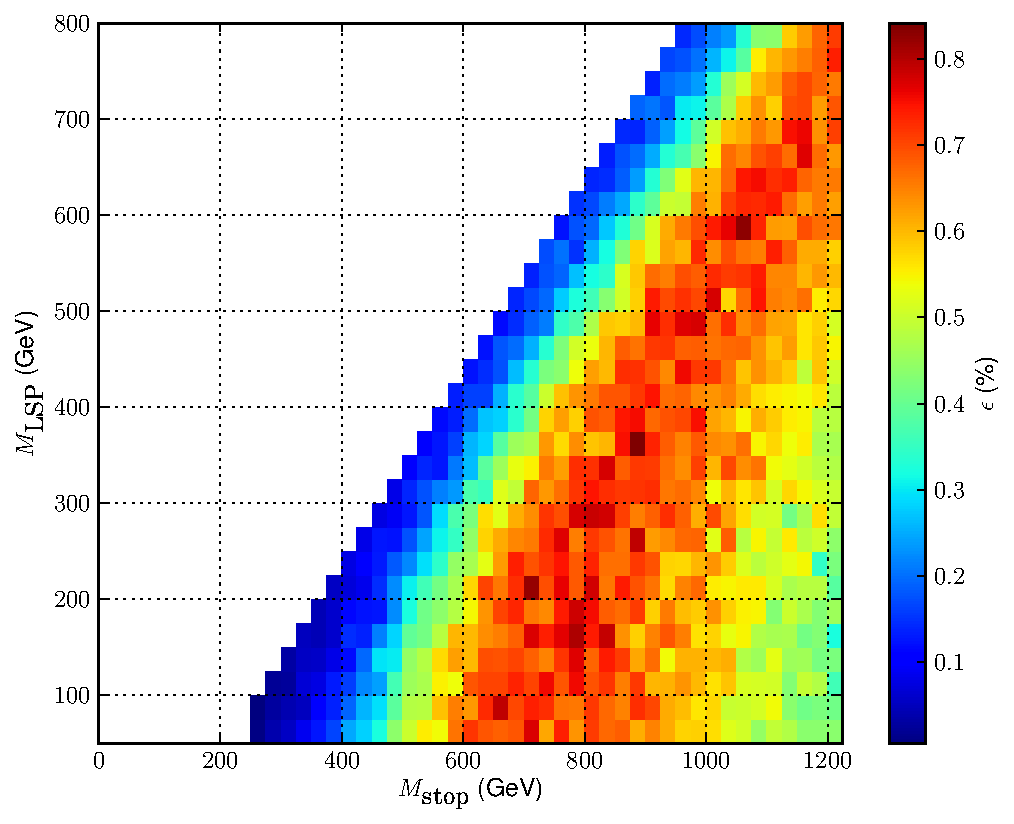
\includegraphics[width=0.49\textwidth]{fig/t2tt_muons_eff_350}}\\
\subfloat[]{\label{fig:inter_t2tt_mu_eff450}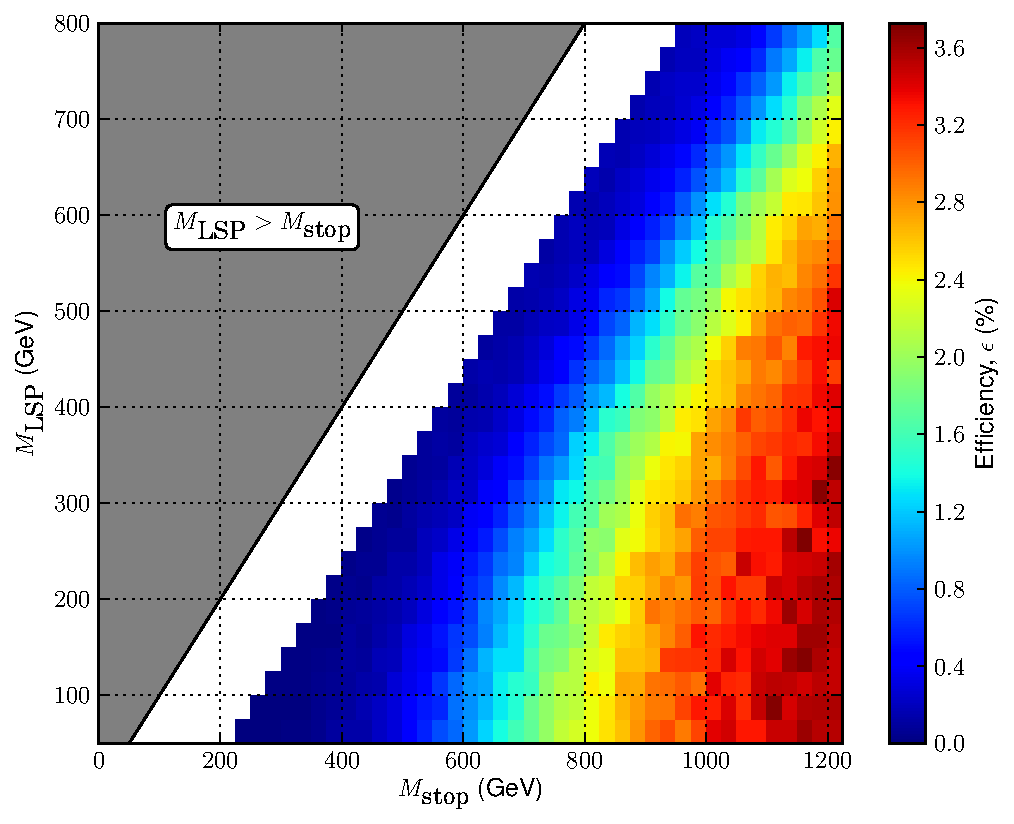
\includegraphics[width=0.49\textwidth]{fig/t2tt_muons_eff_450}}
\subfloat[]{\label{fig:inter_t2tt_mu_efftot}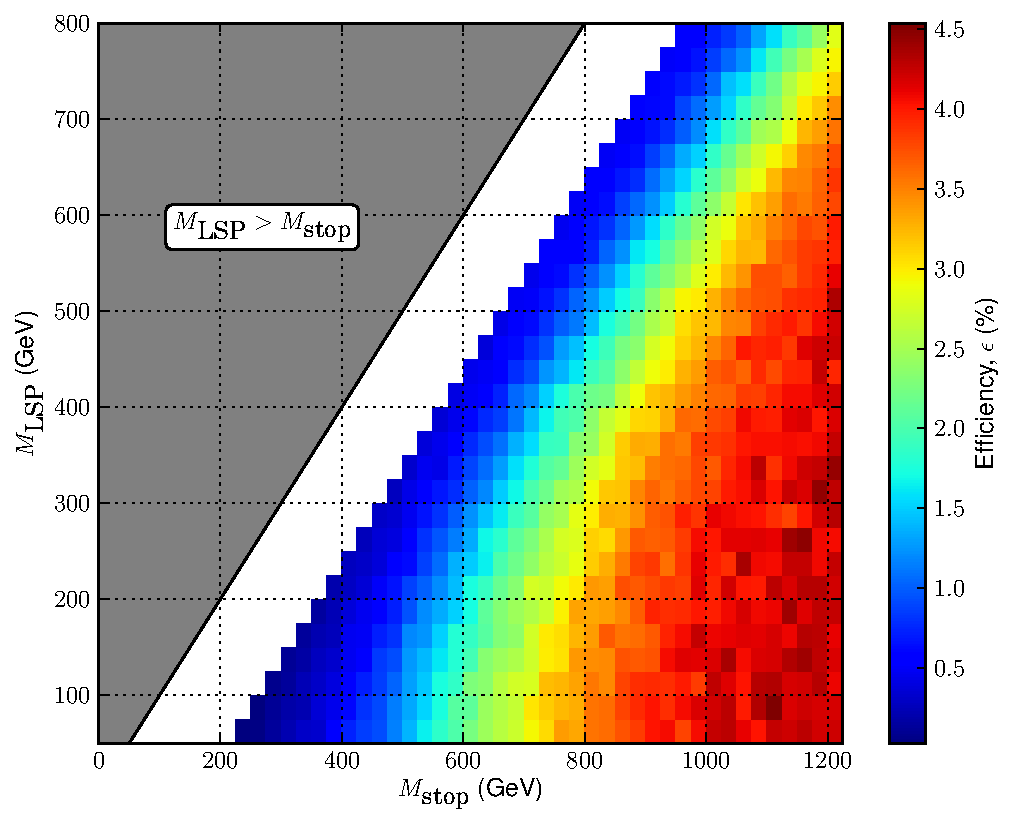
\includegraphics[width=0.49\textwidth]{fig/t2tt_muons_eff_total}}
\caption[]{}
\label{fig:inter_t2tt_mu}
\end{figure}

\begin{figure}[h!]
\centering
\subfloat[]{\label{fig:inter_t2tt_el_eff250}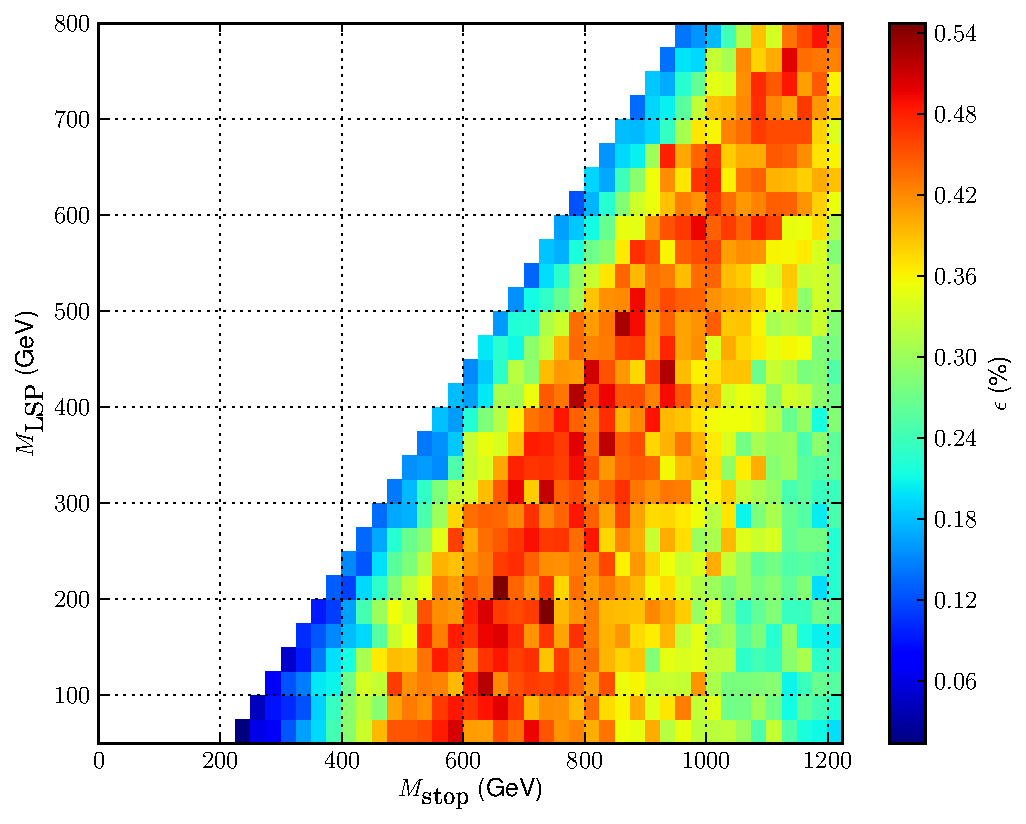
\includegraphics[width=0.49\textwidth]{fig/t2tt_electrons_eff_250}}
\subfloat[]{\label{fig:inter_t2tt_el_eff350}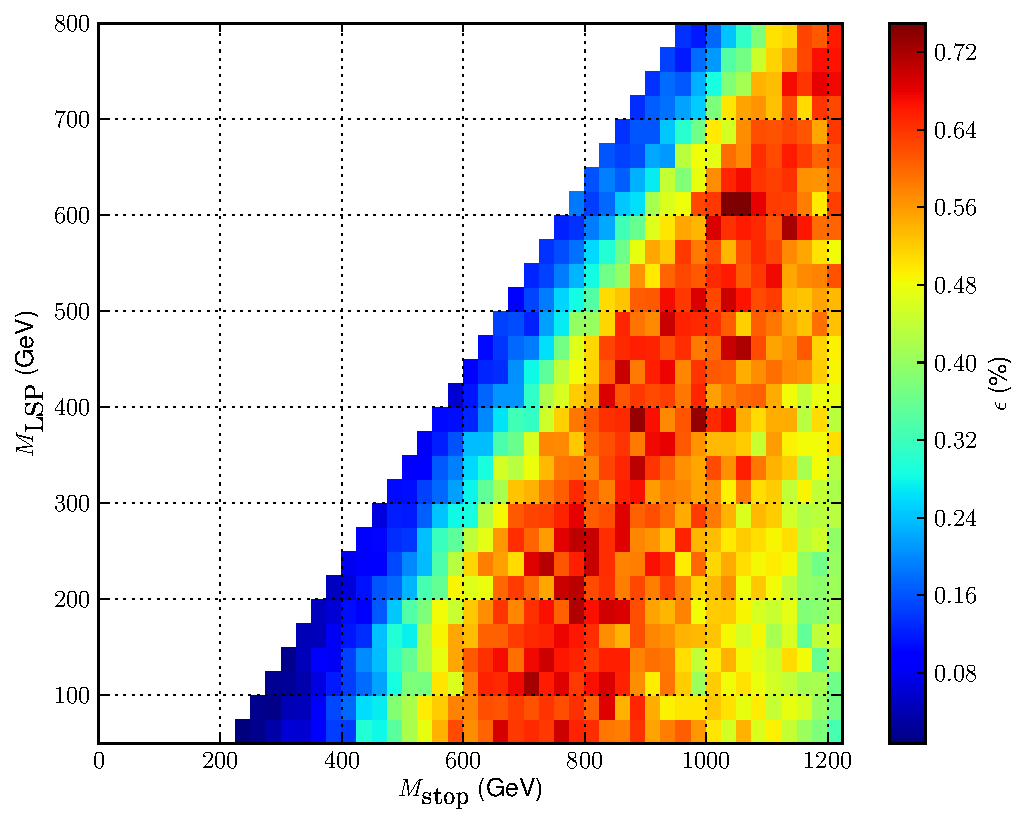
\includegraphics[width=0.49\textwidth]{fig/t2tt_electrons_eff_350}}\\
\subfloat[]{\label{fig:inter_t2tt_el_eff450}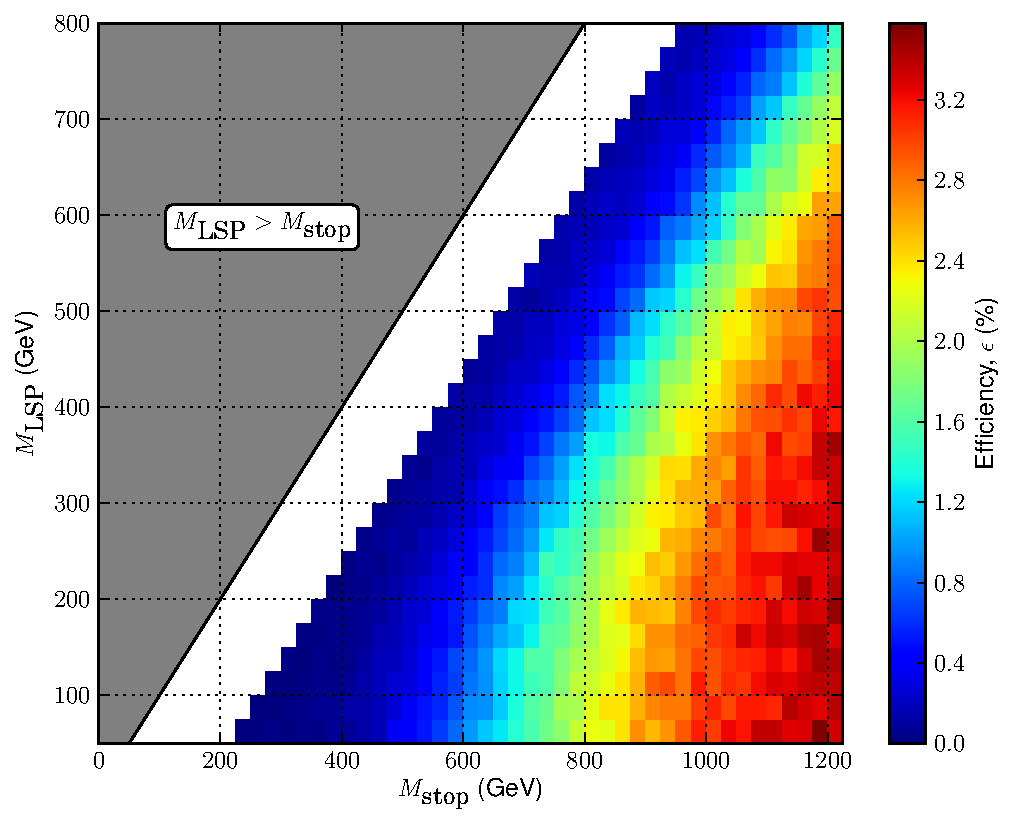
\includegraphics[width=0.49\textwidth]{fig/t2tt_electrons_eff_450}}
\subfloat[]{\label{fig:inter_t2tt_el_efftot}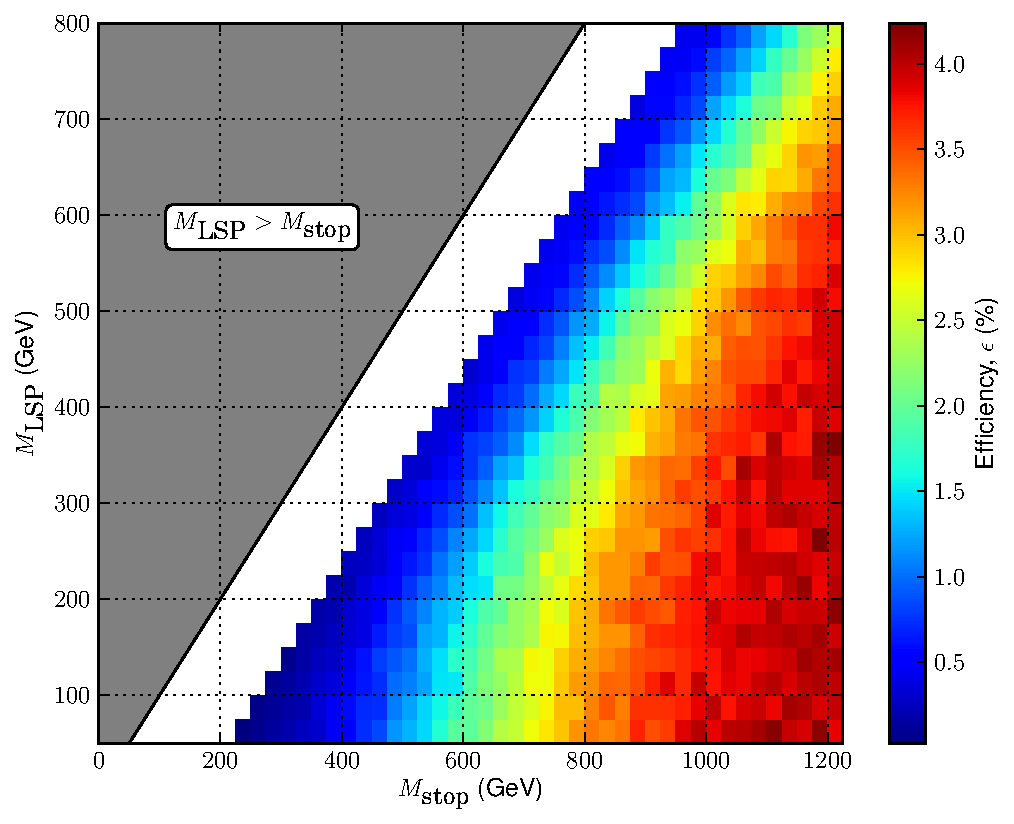
\includegraphics[width=0.49\textwidth]{fig/t2tt_electrons_eff_total}}
\caption[]{}
\label{fig:inter_t2tt_el}
\end{figure}

\begin{figure}[h!]
\centering
\subfloat[]{\label{fig:inter_t2tt_limit}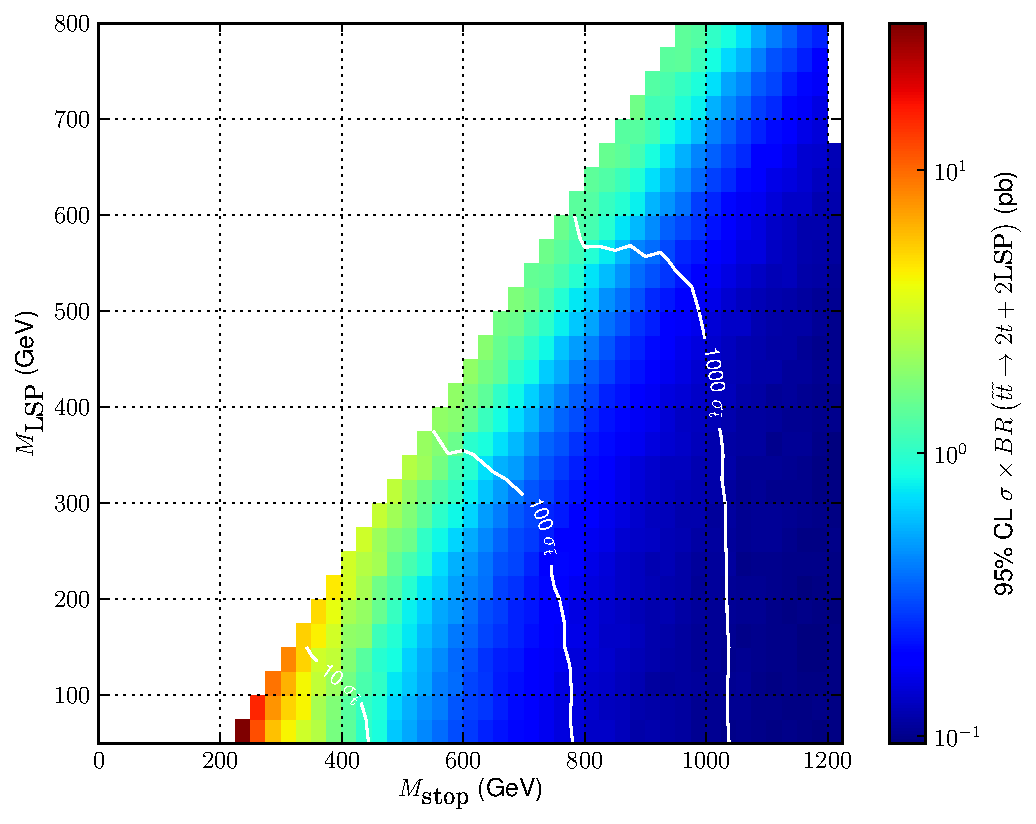
\includegraphics[width=0.49\textwidth]{fig/t2tt_limit}}
\subfloat[]{\label{fig:inter_t2tt_limit_1d}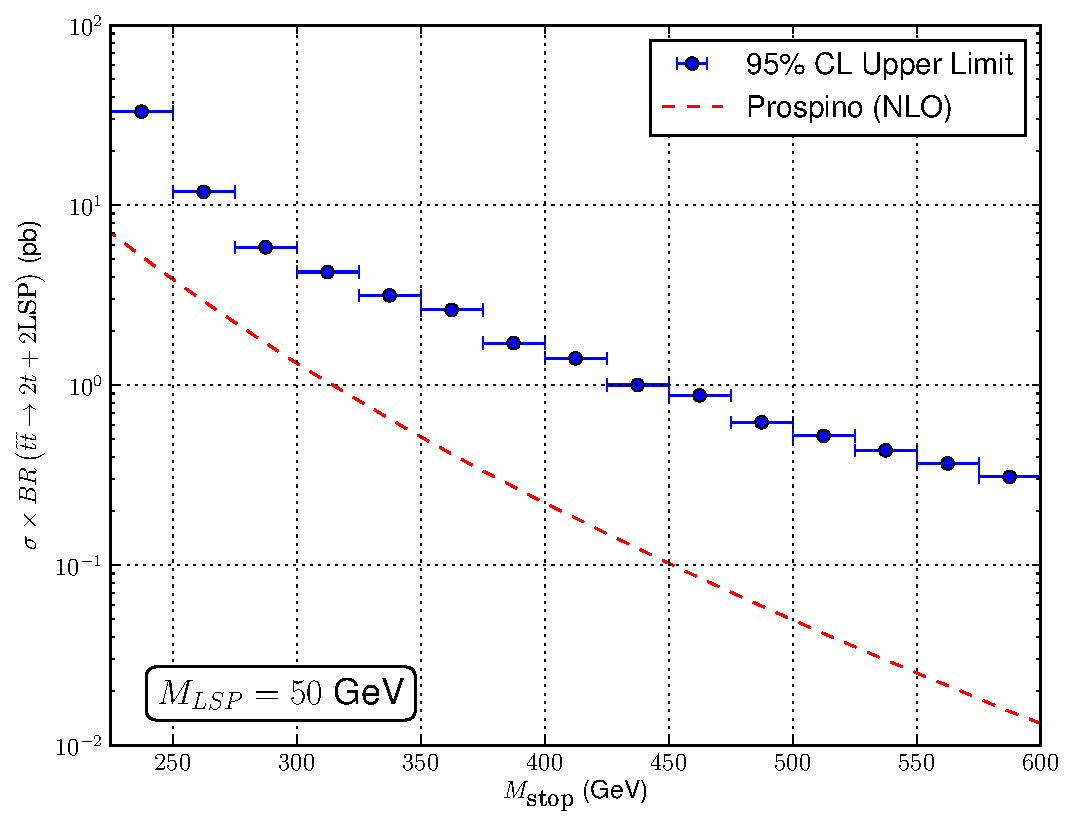
\includegraphics[width=0.49\textwidth]{fig/t2tt_limit_1d}}
\caption[]{}
\label{fig:inter_t2tt}
\end{figure}





%%% Local Variables:
%%% mode: latex
%%% TeX-master: "../thesis"
%%% End:
